\documentclass[]{article}

\usepackage{lmodern}
\usepackage{amssymb,amsmath}
\usepackage{ifxetex,ifluatex}
\usepackage{fixltx2e} % provides \textsubscript
\usepackage[T1]{fontenc}
\usepackage[utf8]{inputenc}
\usepackage{upquote}
\usepackage{microtype}
\usepackage[unicode=true]{hyperref}
\usepackage{longtable,booktabs}
\usepackage{footnote}
\usepackage{listings}
\usepackage{parskip}
\usepackage[margin=0.7in]{geometry}
\usepackage{titlesec}
\usepackage[yyyymmdd,hhmmss]{datetime}
\usepackage{textcomp}
\usepackage{tikz}

\usetikzlibrary{trees}
\tikzstyle{every node}=[draw=black,thick,anchor=west]
\tikzstyle{selected}=[draw=blue]
\tikzstyle{optional}=[dashed,fill=gray!50]

\renewcommand{\dateseparator}{.}

% Newer LaTeX versions should not add ligatures to listings, but for some reason
% it is not the case for me. As a result select PDF viewers copy wrong data.
\lstdefinestyle{ocbash}{
  language=bash,
  frame=tb,
  columns=fullflexible,
  captionpos=b,
  morekeywords={git, make, build, ioreg, grep, nvram, sort, sudo, diskutil, gfxutil, strings, dd, cut},
  literate =
    {"}{{\textquotedbl}}1
    {'}{{\textquotesingle}}1
    {-}{{-}}1
    {~}{{\texttildelow}}1
    {*}{{*}}1
    {fl}{{f{}l}}2
    {fi}{{f{}i}}2
    ,
}

\UseMicrotypeSet[protrusion]{basicmath} % disable protrusion for tt fonts
\PassOptionsToPackage{hyphens}{url} % url is loaded by hyperref

\makesavenoteenv{long table} % Fix footnotes in tables

% set default figure placement to htbp
\makeatletter
\def\fps@figure{htbp}
\makeatother

\providecommand{\tightlist}{%
  \setlength{\itemsep}{0pt}\setlength{\parskip}{0pt}}

\newcommand{\sectionbreak}{\clearpage}

\begin{document}

\begin{titlepage}
   \begin{center}
       \vspace*{3.5in}

       \Huge

       \textbf{OpenCore}

       \vspace{0.2in}

       Reference Manual (0.0.2)

       \vspace{0.2in}

        {[}\today{]}

       \normalsize

       \vfill

       Copyright \textcopyright 2018-2019 vit9696

   \end{center}
\end{titlepage}

\tableofcontents

\section{Introduction}\label{introduction}

This document provides information on
\href{https://github.com/acidanthera/OpenCorePkg}{OpenCore} user
configuration file format used to setup the correct functioning of macOS
operating system.

\subsection{Known defects}\label{reported-defects}

For OpenCore issues please refer to
\href{https://github.com/acidanthera/bugtracker}{Acidanthera Bugtracker}.

\section{Generic Terms}\label{generic-terms}

\begin{itemize}
\item
  \texttt{plist} --- Subset of ASCII Property List format written in
  XML, also know as XML plist format version 1. Uniform Type Identifier
  (UTI): \texttt{com.apple.property-list}. Plists consist of
  \texttt{plist\ objects}, which are combined to form a hierarchical
  structure. Due to plist format not being well-defined, all the
  definitions of this document may only be applied after plist is
  considered valid by running \texttt{plutil\ -lint}. External
  references: https://www.apple.com/DTDs/PropertyList-1.0.dtd,
  \texttt{man\ plutil}.
\item
  \texttt{plist\ type} --- plist collections (\texttt{plist\ array},
  \texttt{plist\ dictionary}, \texttt{plist\ key}) and primitives
  (\texttt{plist\ string}, \texttt{plist\ data}, \texttt{plist\ date},
  \texttt{plist\ boolean}, \texttt{plist\ integer},
  \texttt{plist\ real}).
\item
  \texttt{plist\ object} --- definite realisation of
  \texttt{plist\ type}, which may be interpreted as value.
\item
  \texttt{plist\ array} --- array-like collection, conforms to
  \texttt{array}. Consists of zero or more \texttt{plist\ objects}.
\item
  \texttt{plist\ dictionary} --- map-like (associative array)
  collection, conforms to \texttt{dict}. Consists of zero or more
  \texttt{plist\ keys}.
\item
  \texttt{plist\ key} --- contains one \texttt{plist\ object} going by
  the name of \texttt{plist\ key}, conforms to \texttt{key}. Consists of
  printable 7-bit ASCII characters.
\item
  \texttt{plist\ string} --- printable 7-bit ASCII string, conforms to
  \texttt{string}.
\item
  \texttt{plist\ data} --- base64-encoded blob, conforms to
  \texttt{data}.
\item
  \texttt{plist\ date} --- ISO-8601 date, conforms to \texttt{date},
  unsupported.
\item
  \texttt{plist\ boolean} --- logical state object, which is either true
  (1) or false (0), conforms to \texttt{true} and \texttt{false}.
\item
  \texttt{plist\ integer} --- possibly signed integer number in base 10,
  conforms to \texttt{integer}. Fits in 64-bit unsigned integer in two's
  complement representation, unless a smaller signed or unsigned
  integral type is explicitly mentioned in specific
  \texttt{plist\ object} description.
\item
  \texttt{plist\ real} --- floating point number, conforms to
  \texttt{real}, unsupported.
\item
  \texttt{plist\ metadata} --- value cast to data by the implementation.
  Permits passing \texttt{plist\ string}, in which case the result is
  represented by a null-terminated sequence of bytes (aka C string),
  \texttt{plist\ integer}, in which case the result is represented by
  \emph{32-bit} little endian sequence of bytes in two's complement
  representation, \texttt{plist\ boolean}, in which case the value is
  one byte: \texttt{01} for \texttt{true} and \texttt{00} for
  \texttt{false}, and \texttt{plist\ data} itself. All other types or
  larger integers invoke undefined behaviour.
\end{itemize}

\section{Overview}\label{configuration-overview}

\subsection{Configuration Terms}\label{configuration-terms}

\begin{itemize}
\item
  \texttt{OC\ config} --- OpenCore Configuration file in \texttt{plist}
  format named \texttt{config.plist}. It has to provide extensible way
  to configure OpenCore and is structured to be separated into multiple
  named sections situated in the root \texttt{plist\ dictionary}. These
  sections are permitted to have \texttt{plist\ array} or
  \texttt{plist\ dictionary} types and are described in corresponding
  sections of this document.
\item
  \texttt{valid\ key} --- \texttt{plist\ key} object of
  \texttt{OC\ config} described in this document or its future
  revisions. Besides explicitly described \texttt{valid\ keys}, keys
  starting with \texttt{\#} symbol (e.g. \texttt{\#Hello}) are also
  considered \texttt{valid\ keys} and behave as comments, effectively
  discarding their value, which is still required to be a valid
  \texttt{plist\ object}. All other \texttt{plist\ keys} are not valid,
  and their presence yields to \texttt{undefined\ behaviour}.
\item
  \texttt{valid\ value} --- valid \texttt{plist\ object} of
  \texttt{OC\ config} described in this document that matches all the
  additional requirements in specific \texttt{plist\ object} description
  if any.
\item
  \texttt{invalid\ value} --- valid \texttt{plist\ object} of
  \texttt{OC\ config} described in this document that is of other
  \texttt{plist\ type}, does not conform to additional requirements
  found in specific \texttt{plist\ object} description (e.g.~value
  range), or missing from the corresponding collection.
  \texttt{Invalid\ value} is read with or without an error message as
  any possible value of this \texttt{plist\ object} in an undetermined
  manner (i.e.~the values may not be same across the reboots). Whilst
  reading an \texttt{invalid\ value} is equivalent to reading certain
  defined \texttt{valid\ value}, applying incompatible value to the host
  system may yield to \texttt{undefined\ behaviour}.
\item
  \texttt{optional\ value} --- \texttt{valid\ value} of
  \texttt{OC\ config} described in this document that reads in a certain
  defined manner provided in specific \texttt{plist\ object} description
  (instead of \texttt{invalid\ value}) when not present in
  \texttt{OC\ config}. All other cases of \texttt{invalid\ value} do
  still apply. Unless explicitly marked as \texttt{optional\ value}, any
  other value is required to be present and reads to
  \texttt{invalid\ value} if missing.
\item
  \texttt{fatal\ behaviour} --- behaviour leading to boot termination.
  Implementation must stop the boot process from going any further until
  next host system boot. It is allowed but not required to perform cold
  reboot or show any warning message.
\item
  \texttt{undefined\ behaviour} --- behaviour not prescribed by this
  document. Implementation is allowed to take any measures including but
  not limited to \texttt{fatal\ behaviour}, assuming any states or
  values, or ignoring, unless these measures negatively affect system
  security in general.
\end{itemize}

\subsection{Configuration Processing}\label{configuration-processing}

\texttt{OC\ config} is guaranteed to be processed at least once if it
was found. Depending on OpenCore bootstrapping mechanism multiple
\texttt{OC\ config} files may lead to reading any of them. No
\texttt{OC\ Config} may be present on disk, in which case all the values
read follow the rules of \texttt{invalid\ value} and
\texttt{optional\ value}.

\texttt{OC\ config} has size, nesting, and key amount limitations.
\texttt{OC\ config} size does not exceed \texttt{16\ MBs}.
\texttt{OC\ config} has no more than \texttt{8} nesting levels.
\texttt{OC\ config} has up to \texttt{16384} XML nodes (i.e.~one
\texttt{plist\ dictionary} item is counted as a pair of nodes) within
each \texttt{plist\ object}.

Reading malformed \texttt{OC\ config} file leads to
\texttt{undefined\ behaviour}. Examples of malformed \texttt{OC\ config}
cover at least the following cases:

\begin{itemize}
\tightlist
\item
  files non-conformant to \texttt{plist} DTD
\item
  files with unsupported or non-conformant \texttt{plist\ objects} found
  in this document
\item
  files violating size, nesting, and key amount limitations
\end{itemize}

It is recommended but not required to abort loading malformed
\texttt{OC\ config} and continue as if no \texttt{OC\ config} was
present. For forward compatibility it is recommended but not required
for the implementation to warn about the use of
\texttt{invalid\ values}. Recommended practice of interpreting
\texttt{invalid\ values} is to conform to the following convention where
applicable:

\begin{longtable}[]{@{}ll@{}}
\toprule
Type & Value\tabularnewline
\midrule
\endhead
\texttt{plist\ string} & Empty string
(\texttt{\textless{}string\textgreater{}\textless{}/string\textgreater{}})\tabularnewline
\texttt{plist\ data} & Empty data
(\texttt{\textless{}data\textgreater{}\textless{}/data\textgreater{}})\tabularnewline
\texttt{plist\ integer} & 0
(\texttt{\textless{}integer\textgreater{}0\textless{}/integer\textgreater{}})\tabularnewline
\texttt{plist\ boolean} & False
(\texttt{\textless{}false/\textgreater{}})\tabularnewline
\texttt{plist\ tristate} & False
(\texttt{\textless{}false/\textgreater{}})\tabularnewline
\bottomrule
\end{longtable}

\subsection{Configuration Structure}\label{configuration-structure}

\texttt{OC\ config} is separated into following sections, which are described
in separate sections of this document. By default it is tried to not enable
anything and optionally provide kill switches with \texttt{Enable} property
for \texttt{plist dict} entries. In general the configuration is written
idiomatically to group similar actions in subsections:

\begin{itemize}
\tightlist
\item
  \texttt{Add} provides support for data addition.
\item
  \texttt{Block} provides support for data removal or ignorance.
\item
  \texttt{Patch} provides support for data modification.
\item
  \texttt{Quirks} provides support for specific hacks.
\end{itemize}

Root configuration entries consist of the following:

\begin{itemize}
\tightlist
\item
  \hyperref[acpi]{\texttt{ACPI}}
\item
  \hyperref[devprops]{\texttt{DeviceProperties}}
\item
  \hyperref[kernel]{\texttt{Kernel}}
\item
  \hyperref[misc]{\texttt{Misc}}
\item
  \hyperref[nvram]{\texttt{NVRAM}}
\item
  \hyperref[platforminfo]{\texttt{PlatformInfo}}
\item
  \hyperref[uefi]{\texttt{UEFI}}
\end{itemize}

\emph{Note}: Currently most properties try to have defined values even if not
specified in the configuration for safety reasons. This behaviour should not
be relied upon, and all fields must be properly specified in the configuration.

\subsection{Directory Structure}\label{directory-structure}

When directory boot is used the directory structure used should follow
the description on \hyperref[fig:DS]{Directory Structure} figure. Available
entries include:

\begin{itemize}
\tightlist
\item
  \texttt{BOOTx64.efi}
  \break
  Initial booter, which loads \texttt{OpenCore.efi} unless it was
  already started as a driver.
\item
  \texttt{ACPI}
  \break
  Directory used for storing supplemental ACPI information
  for \hyperref[acpi]{\texttt{ACPI}} section.
\item
  \texttt{Drivers}
  \break
  Directory used for storing supplemental \texttt{UEFI}
  drivers for \hyperref[uefi]{\texttt{UEFI}} section.
\item
  \texttt{Kexts}
  \break
  Directory used for storing supplemental kernel information
  for \hyperref[kernel]{\texttt{Kernel}} section.
\item
  \texttt{OpenCore.efi}
  \break
  Main booter driver responsible for operating system loading.
\item
  \texttt{vault.plist}
  \break
  Hashes for all files potentially loadable by \texttt{OC Config}.
\item
  \texttt{config.plist}
  \break
  \texttt{OC Config}.
\item
  \texttt{vault.sig}
  \break
  Signature for \texttt{vault.plist}.
\end{itemize}

\begin{center}
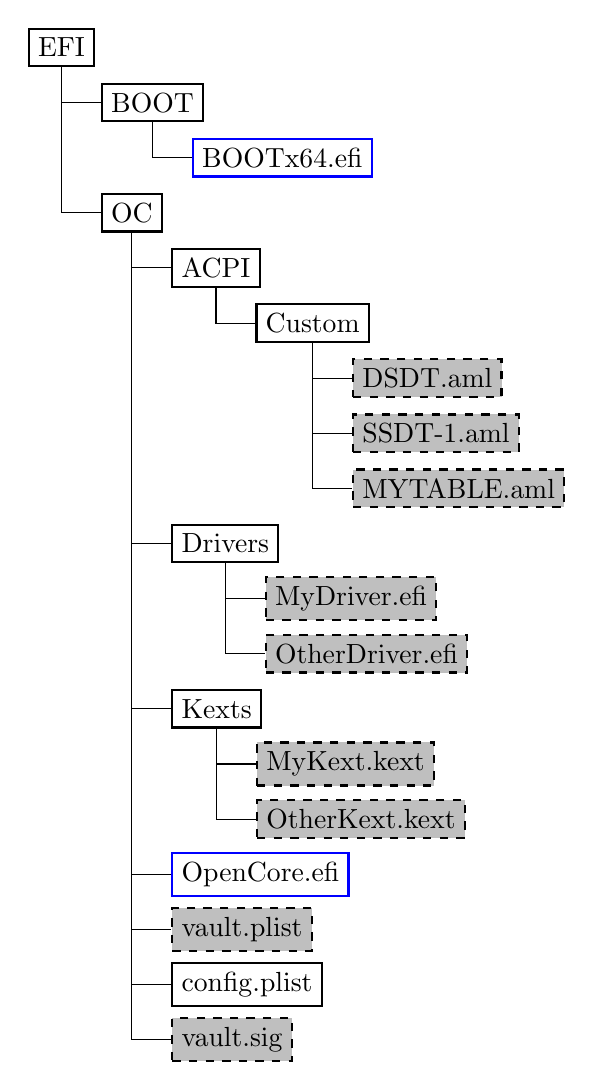
\begin{tikzpicture}[%
  grow via three points={one child at (0.5,-0.7) and
  two children at (0.5,-0.7) and (0.5,-1.4)},
  edge from parent path={(\tikzparentnode.south) |- (\tikzchildnode.west)}]
  \node {EFI}
    child { node {BOOT}
      child { node [selected] {BOOTx64.efi}}
    }
    child [missing] {}
    child { node {OC}
      child { node {ACPI}
        child { node {Custom}
          child { node [optional] {DSDT.aml}}
          child { node [optional] {SSDT-1.aml}}
          child { node [optional] {MYTABLE.aml}}
        }
      }
      child [missing] {}
      child [missing] {}
      child [missing] {}
      child [missing] {}
      child { node {Drivers}
        child { node [optional] {MyDriver.efi}}
        child { node [optional] {OtherDriver.efi}}
      }
      child [missing] {}
      child [missing] {}
      child { node {Kexts}
        child { node [optional] {MyKext.kext}}
        child { node [optional] {OtherKext.kext}}
      }
      child [missing] {}
      child [missing] {}
      child { node [selected] {OpenCore.efi}}
      child { node [optional] {vault.plist}}
      child { node {config.plist}}
      child { node [optional] {vault.sig}}
    };
\end{tikzpicture}
\break
\label{fig:DS}
Figure 1. Directory Structure
\end{center}

\subsection{Contribution}\label{configuration-comp}

OpenCore can be compiled as an ordinary EDK II package with
\href{https://github.com/tianocore/tianocore.github.io/wiki/UDK2018}{UDK 2018}.

The only officially supported toolchain is \texttt{XCODE5}. Other toolchains
might work, but are neither supported, nor recommended. Contribution of clean
patches is welcome. Please do follow
\href{https://github.com/tianocore/tianocore.github.io/wiki/Code-Style-C}{EDK II C Codestyle}.

Required external package dependencies include
\href{https://github.com/acidanthera/OcSupportPkg}{EfiPkg},
\href{https://github.com/acidanthera/OcSupportPkg}{MacInfoPkg}, and
\href{https://github.com/acidanthera/OcSupportPkg}{OcSupportPkg}.

To compile with \texttt{XCODE5}, besides \href{https://developer.apple.com/xcode}{Xcode},
one should also install \href{https://www.nasm.us}{NASM} and
\href{https://github.com/acidanthera/ocbuild/raw/master/external/mtoc-mac64.zip}{MTOC}. Example command sequence may look as follows:

\begin{lstlisting}[caption=Compilation Commands, label=compile, style=ocbash]
git clone https://github.com/tianocore/edk2 -b UDK2018 UDK
cd UDK
git clone https://github.com/acidanthera/EfiPkg
git clone https://github.com/acidanthera/MacInfoPkg
git clone https://github.com/acidanthera/OcSupportPkg
git clone https://github.com/acidanthera/OpenCorePkg
source edksetup.sh
make -C BaseTools
build -a X64 -b RELEASE -t XCODE5 -p OpenCorePkg/OpenCorePkg.dsc
\end{lstlisting}

\texttt{NOOPT} or \texttt{DEBUG} build modes instead of \texttt{RELEASE}
can produce a lot more debug output. With \texttt{NOOPT} source level debugging with
GDB or IDA Pro is also available. For GDB check
\href{https://github.com/acidanthera/OcSupportPkg/tree/master/Debug}{OcSupport Debug}
page. For IDA Pro you will need IDA Pro 7.3 or newer.

For IDE usage Xcode projects are available in the root of the repositories. Another
approach could be \href{https://www.sublimetext.com}{Sublime Text} with
\href{https://niosus.github.io/EasyClangComplete}{EasyClangComplete} plugin.
Add \texttt{.clang\_complete} file with similar content to your UDK root:

\begin{lstlisting}[caption=ECC Configuration, label=eccfile, style=ocbash]
-I/UefiPackages/MdePkg
-I/UefiPackages/MdePkg/Include
-I/UefiPackages/MdePkg/Include/X64
-I/UefiPackages/EfiPkg
-I/UefiPackages/EfiPkg/Include
-I/UefiPackages/EfiPkg/Include/X64
-I/UefiPackages/AptioFixPkg/Include
-I/UefiPackages/AppleSupportPkg/Include
-I/UefiPackages/OpenCorePkg/Include
-I/UefiPackages/OcSupportPkg/Include
-I/UefiPackages/IntelFrameworkPkg/Include
-I/UefiPackages/MacInfoPkg/Include
-IInclude
-include
/UefiPackages/MdePkg/Include/Uefi.h
-fshort-wchar
-Wall
-Wextra
-Wno-unused-parameter
-Wno-missing-braces
-Wno-missing-field-initializers
-Wno-tautological-compare
-Wno-sign-compare
-Wno-varargs
-Wno-unused-const-variable
\end{lstlisting}

\textbf{Warning}: Tool developers modifying \texttt{config.plist} or any other OpenCore
files must ensure that their tool checks for \texttt{opencore-version} NVRAM variable
(see \hyperref[miscdebugprops]{Debug Properties} section below) and warn the user
if the version listed is unsupported or prerelease. OpenCore configuration may change
across the releases and the tool shall ensure that it carefully follows this document.
Failure to do so may result in this tool to be considered as malware and blocked with
all possible means.

\section{ACPI}\label{acpi}

\subsection{Introduction}\label{acpiintro}

ACPI (Advanced Configuration and Power Interface) is an open standard to
discover and configure computer hardware.
\href{https://uefi.org/specifications}{ACPI specification} defines the
standard tables (e.g.~\texttt{DSDT}, \texttt{SSDT}, \texttt{FACS}, \texttt{DMAR})
and various methods (e.g. \texttt{\_DSM}, \texttt{\_PWR}) for implementation.
Modern hardware needs little changes to maintain ACPI compatibility, yet
some of those are provided as a part of OpenCore.

\subsection{Properties}\label{acpiprops}

\begin{enumerate}
\item
  \texttt{Add}\\
  \textbf{Type}: \texttt{plist\ array}\\
  \textbf{Default value}: Empty\\
  \textbf{Description}: Load selected tables from \texttt{OC/ACPI/Custom}
  directory.

  Designed to be filled with \texttt{plist\ dict} values, describing each block entry.
  See \hyperref[acpipropsadd]{Add Properties} section below.

\item
  \texttt{Block}\\
  \textbf{Type}: \texttt{plist\ array}\\
  \textbf{Default value}: Empty\\
  \textbf{Description}: Remove selected tables from ACPI stack.

  Designed to be filled with \texttt{plist\ dict} values, describing each block entry.
  See \hyperref[acpipropsblock]{Block Properties} section below.

\item
  \texttt{Patch}\\
  \textbf{Type}: \texttt{plist\ array}\\
  \textbf{Default value}: Empty\\
  \textbf{Description}: Perform binary patches in ACPI tables before
  table addition or removal.

  Designed to be filled with \texttt{plist\ dictionary} values describing each
  patch entry. See \hyperref[acpipropspatch]{Patch Properties} section below.

\item
  \texttt{Quirks}\\
  \textbf{Type}: \texttt{plist\ dict}\\
  \textbf{Description}: Apply individual ACPI quirks described
  in \hyperref[acpipropsquirks]{Quirks Properties} section below.

\end{enumerate}

\subsection{Add Properties}\label{acpipropsadd}

\begin{enumerate}
\item
  \texttt{Comment}\\
  \textbf{Type}: \texttt{plist\ string}\\
  \textbf{Default value}: Empty string\\
  \textbf{Description}: Arbitrary ASCII string used to provide human readable
  reference for the entry. It is implementation defined whether this value is
  used.

\item
  \texttt{Enabled}\\
  \textbf{Type}: \texttt{plist\ boolean}\\
  \textbf{Default value}: \texttt{false}\\
  \textbf{Description}: This ACPI table will not be added unless set to
  \texttt{true}.

\item
  \texttt{Path}\\
  \textbf{Type}: \texttt{plist\ string}\\
  \textbf{Default value}: Empty string\\
  \textbf{Description}: File paths meant to be loaded as ACPI tables.
  Example values include \texttt{DSDT.aml}, \texttt{SubDir/SSDT-8.aml},
  \texttt{SSDT-USBX.aml}, etc.

  ACPI table load order follows the item order in the array. All ACPI tables
  load from \texttt{OC/ACPI/Custom} directory.

  \textbf{Note}: All tables but tables with \texttt{DSDT} table identifier
  (determined by parsing data not by filename) insert new tables into ACPI stack.
  \texttt{DSDT}, unlike the rest, performs replacement of DSDT table.

\end{enumerate}

\subsection{Block Properties}\label{acpipropsblock}

\begin{enumerate}
\item
  \texttt{All}\\
  \textbf{Type}: \texttt{plist\ boolean}\\
  \textbf{Default value}: \texttt{false}\\
  \textbf{Description}: If set to \texttt{true}, all ACPI tables matching the
  condition will be dropped. Otherwise only first matched table.

\item
  \texttt{Comment}\\
  \textbf{Type}: \texttt{plist\ string}\\
  \textbf{Default value}: Empty string\\
  \textbf{Description}: Arbitrary ASCII string used to provide human readable
  reference for the entry. It is implementation defined whether this value is
  used.

\item
  \texttt{Enabled}\\
  \textbf{Type}: \texttt{plist\ boolean}\\
  \textbf{Default value}: \texttt{false}\\
  \textbf{Description}: This ACPI table will not be removed unless set to
  \texttt{true}.

\item
  \texttt{OemTableId}\\
  \textbf{Type}: \texttt{plist\ data}, 8 bytes\\
  \textbf{Default value}: All zero\\
  \textbf{Description}: Match table OEM ID to be equal to this value
  unless all zero.

\item
  \texttt{TableLength}\\
  \textbf{Type}: \texttt{plist\ integer}\\
  \textbf{Default value}: \texttt{0}\\
  \textbf{Description}: Match table size to be equal to this value
  unless \texttt{0}.

\item
  \texttt{TableSignature}\\
  \textbf{Type}: \texttt{plist\ data}, 4 bytes\\
  \textbf{Default value}: All zero\\
  \textbf{Description}: Match table signature to be equal to this value
  unless all zero.

\end{enumerate}

\subsection{Patch Properties}\label{acpipropspatch}

\begin{enumerate}

\item
  \texttt{Comment}\\
  \textbf{Type}: \texttt{plist\ string}\\
  \textbf{Default value}: Empty string\\
  \textbf{Description}: Arbitrary ASCII string used to provide human readable
  reference for the entry. It is implementation defined whether this value is
  used.

\item
  \texttt{Count}\\
  \textbf{Type}: \texttt{plist\ integer}\\
  \textbf{Default value}: \texttt{0}\\
  \textbf{Description}: Number of patch occurrences to apply. \texttt{0} applies
  the patch to all occurrences found.

\item
  \texttt{Enabled}\\
  \textbf{Type}: \texttt{plist\ boolean}\\
  \textbf{Default value}: \texttt{false}\\
  \textbf{Description}: This ACPI patch will not be used unless set to
  \texttt{true}.

\item
  \texttt{Find}\\
  \textbf{Type}: \texttt{plist\ data}\\
  \textbf{Default value}: Empty data\\
  \textbf{Description}: Data to find. Must equal to \texttt{Replace} in size.

\item
  \texttt{Limit}\\
  \textbf{Type}: \texttt{plist\ integer}\\
  \textbf{Default value}: \texttt{0}\\
  \textbf{Description}: Maximum number of bytes to search for. Can be set to
  \texttt{0} to look through the whole ACPI table.

\item
  \texttt{Mask}\\
  \textbf{Type}: \texttt{plist\ data}\\
  \textbf{Default value}: Empty data\\
  \textbf{Description}: Data bitwise mask used during find comparison.
  Allows fuzzy search by ignoring not masked (set to zero) bits. Can be
  set to empty data to be ignored. Must equal to \texttt{Replace} in size
  otherwise.

\item
  \texttt{OemTableId}\\
  \textbf{Type}: \texttt{plist\ data}, 8 bytes\\
  \textbf{Default value}: All zero\\
  \textbf{Description}: Match table OEM ID to be equal to this value
  unless all zero.

\item
  \texttt{Replace}\\
  \textbf{Type}: \texttt{plist\ data}\\
  \textbf{Default value}: Empty data\\
  \textbf{Description}: Replacement data of one or more bytes.

\item
  \texttt{ReplaceMask}\\
  \textbf{Type}: \texttt{plist\ data}\\
  \textbf{Default value}: Empty data\\
  \textbf{Description}: Data bitwise mask used during replacement.
  Allows fuzzy replacement by updating masked (set to non-zero) bits. Can be
  set to empty data to be ignored. Must equal to \texttt{Replace} in size
  otherwise.

\item
  \texttt{Skip}\\
  \textbf{Type}: \texttt{plist\ integer}\\
  \textbf{Default value}: \texttt{0}\\
  \textbf{Description}: Number of found occurrences to be skipped before replacement
  is done.

\item
  \texttt{TableLength}\\
  \textbf{Type}: \texttt{plist\ integer}\\
  \textbf{Default value}: \texttt{0}\\
  \textbf{Description}: Match table size to be equal to this value
  unless \texttt{0}.

\item
  \texttt{TableSignature}\\
  \textbf{Type}: \\texttt{plist\ data}, 4 bytes\\
  \textbf{Default value}: All zero\\
  \textbf{Description}: Match table signature to be equal to this value
  unless all zero.

\end{enumerate}

In the majority of the cases ACPI patches are not useful and harmful:

\begin{itemize}
\item
  Avoid renaming devices with ACPI patches. This may fail or perform
  improper renaming of unrelated devices (e.g. \texttt{EC} and
  \texttt{EC0}), be unnecessary, or even fail to rename devices in select tables. For
  ACPI consistency it is much safer to rename devices at I/O Registry
  level, as done by
  \href{https://github.com/acidanthera/WhateverGreen}{WhateverGreen}.
\item
  Avoid patching \texttt{\_OSI} to support a higher level of feature sets
  unless absolutely required. Commonly this enables a number of hacks on APTIO
  firmwares, which result in the need to add more patches. Modern firmwares
  generally do not need it at all, and those that do are fine with much
  smaller patches.
\item
  Try to avoid hacky changes like renaming \texttt{\_PWR} or \texttt{\_DSM}
  whenever possible.
\end{itemize}

Several cases, where patching actually does make sense, include:

\begin{itemize}
\item
  Refreshing \texttt{HPET} (or another device) method header to avoid
  compatibility checks by \texttt{\_OSI} on legacy hardware. \texttt{\_STA}
  method with \texttt{if ((OSFL () == Zero)) \{ If (HPTE)  ...  Return (Zero)}
  content may be forced to always return 0xF by replacing
  \texttt{A0 10 93 4F 53 46 4C 00} with \texttt{A4 0A 0F A3 A3 A3 A3 A3}.
\item
  To provide custom method implementation with in an SSDT, for instance,
  to report functional key presses on a laptop, the original method can be replaced
  with a dummy name by patching \texttt{\_Q11} with \texttt{XQ11}.
\end{itemize}

Tianocore \href{https://github.com/tianocore/edk2/blob/UDK2018/MdePkg/Include/IndustryStandard/AcpiAml.h}{AcpiAml.h}
source file may help understanding ACPI opcodes.

\subsection{Quirks Properties}\label{acpipropsquirks}

\begin{enumerate}

\item
  \texttt{FadtEnableReset}\\
  \textbf{Type}: \texttt{plist\ boolean}\\
  \textbf{Default value}: \texttt{false}\\
  \textbf{Description}: Provide reset register and flag in FADT table to enable
  reboot and shutdown on legacy hardware. Not recommended unless required.

\item
  \texttt{IgnoreForWindows}\\
  \textbf{Type}: \texttt{plist\ boolean}\\
  \textbf{Default value}: \texttt{false}\\
  \textbf{Description}: Disable all sorts of ACPI modifications when booting
  Windows operating system.

  This flag implements a quick workaround for those, who made their ACPI tables
  incompatible with Windows, but need it right now. Not recommended, as ACPI
  tables must be compatible with any operating system regardless of the changes.

  \emph{Note}: This option may be removed in the future.

\item
  \texttt{NormalizeHeaders}\\
  \textbf{Type}: \texttt{plist\ boolean}\\
  \textbf{Default value}: \texttt{false}\\
  \textbf{Description}: Cleanup ACPI header fields to workaround macOS
  ACPI implementation bug causing boot crashes. Reference:
  \href{https://alextjam.es/debugging-appleacpiplatform/}{Debugging
  AppleACPIPlatform on 10.13} by Alex James aka theracermaster. The
  issue is fixed in macOS Mojave (10.14).

\item
  \texttt{RebaseRegions}\\
  \textbf{Type}: \texttt{plist\ boolean}\\
  \textbf{Default value}: \texttt{false}\\
  \textbf{Description}: Attempt to heuristically relocate ACPI memory
  regions. Not recommended.

  ACPI tables are often generated dynamically by underlying firmware
  implementation. Among the position-independent code, ACPI tables may
  contain physical addresses of MMIO areas used for device
  configuration, usually grouped in regions (e.g.
  \texttt{OperationRegion}). Changing firmware settings or hardware
  configuration, upgrading or patching the firmware inevitably leads to
  changes in dynamically generated ACPI code, which sometimes lead to
  the shift of the addresses in aforementioned \texttt{OperationRegion}
  constructions.

  For this reason it is very dangerous to apply any kind of
  modifications to ACPI tables. The most reasonable approach is to make
  as few as possible changes to ACPI and try to not replace any tables,
  especially DSDT. When this is not possible, then at least attempt to
  ensure that custom DSDT is based on the most recent DSDT or remove
  writes and reads for the affected areas.

  When nothing else helps this option could be tried to avoid stalls at
  \texttt{PCI\ Configuration\ Begin} phase of macOS booting by
  attempting to fix the ACPI addresses. It does not do magic, and only
  works with most common cases. Do not use unless absolutely required.

\item
  \texttt{ResetLogoStatus}\\
  \textbf{Type}: \texttt{plist\ boolean}\\
  \textbf{Default value}: \texttt{false}\\
  \textbf{Description}: Reset \texttt{BGRT} table \texttt{Displayed}
  status field to \texttt{false}.

  This works around firmwares that provide \texttt{BGRT} table but
  fail to handle screen updates afterwards.

\end{enumerate}


\section{DeviceProperties}\label{devprops}

\subsection{Introduction}\label{devpropsintro}

Device configuration is provided to macOS with a dedicated buffer,
called \texttt{EfiDevicePropertyDatabase}. This buffer is a serialised
map of DevicePaths to a map of property names and their values.

Property data can be debugged with
\href{https://github.com/acidanthera/gfxutil}{gfxutil}.
To obtain current property data use the following command in macOS:
\begin{lstlisting}[label=gfxutil, style=ocbash]
ioreg -lw0 -p IODeviceTree -n efi -r -x | grep device-properties |
  sed 's/.*<//;s/>.*//' > /tmp/device-properties.hex &&
  gfxutil /tmp/device-properties.hex /tmp/device-properties.plist &&
  cat /tmp/device-properties.plist
\end{lstlisting}

\subsection{Properties}\label{devpropsprops}

\begin{enumerate}
\item
  \texttt{Add}\\
  \textbf{Type}: \texttt{plist\ dict}\\
  \textbf{Description}: Sets device properties from a map (\texttt{plist\ dict})
  of deivce paths to a map (\texttt{plist\ dict}) of variable names and their values
  in \texttt{plist\ metadata} format. Device paths must be provided in canonic string
  format (e.g. \texttt{PciRoot(0x0)/Pci(0x1,0x0)/Pci(0x0,0x0)}). Properties will only
  be set if not present and not blocked.

  \emph{Note}: Currently properties may only be (formerly) added by the original driver,
  so unless a separate driver was installed, there is no reason to block the variables.

\item
  \texttt{Block}\\
  \textbf{Type}: \texttt{plist\ dict}\\
  \textbf{Description}: Removes device properties from a map (\texttt{plist\ dict})
  of deivce paths to an array (\texttt{plist\ array}) of variable names in
  \texttt{plist\ string} format.

\end{enumerate}

\subsection{Common Properties}\label{devpropscommon}

Some known properties include:

\begin{itemize}
\tightlist
\item
  \texttt{device-id}
  \break
  User-specified device identifier used for I/O Kit matching. Has 4 byte data type.
\item
  \texttt{vendor-id}
  \break
  User-specified vendor identifier used for I/O Kit matching. Has 4 byte data type.
\item
  \texttt{AAPL,ig-platform-id}
  \break
  Intel GPU framebuffer identifier used for framebuffer selection on Ivy Bridge and newer.
  Has 4 byte data type.
\item
  \texttt{AAPL,snb-platform-id}
  \break
  Intel GPU framebuffer identifier used for framebuffer selection on Sandy Bridge.
  Has 4 byte data type.
\item
  \texttt{layout-id}
  \break
  Audio layout used for AppleHDA layout selection. Has 4 byte data type.
\end{itemize}


\section{Kernel}\label{kernel}

\subsection{Introduction}\label{kernelintro}

This section allows to apply different kinds of kernelspace modifications on
Apple Kernel (\href{https://opensource.apple.com/source/xnu}{XNU}). The modifications
currently provide driver (kext) injection, kernel and driver patching, and driver
blocking.

\subsection{Properties}\label{kernelprops}

\begin{enumerate}
\item
  \texttt{Add}\\
  \textbf{Type}: \texttt{plist\ array}\\
  \textbf{Default value}: Empty\\
  \textbf{Description}: Load selected kernel drivers from \texttt{OC/Kexts} directory.

  Designed to be filled with \texttt{plist\ dict} values, describing each driver.
  See \hyperref[kernelpropsadd]{Add Properties} section below. Kernel driver load
  order follows the item order in the array, thus the dependencies should be written
  prior to their consumers.

\item
  \texttt{Block}\\
  \textbf{Type}: \texttt{plist\ array}\\
  \textbf{Default value}: Empty\\
  \textbf{Description}: Remove selected kernel drivers from prelinked kernel.

  Designed to be filled with \texttt{plist\ dictionary} values, describing each
  blocked driver. See \hyperref[kernelpropsblock]{Block Properties} section below.

\item
  \texttt{Patch}\\
  \textbf{Type}: \texttt{plist\ array}\\
  \textbf{Default value}: Empty\\
  \textbf{Description}: Perform binary patches in kernel and drivers prior to
  driver addition and removal.

  Designed to be filled with \texttt{plist\ dictionary} values, describing each
  patch. See \hyperref[kernelpropspatch]{Patch Properties} section below.

\item
  \texttt{Quirks}\\
  \textbf{Type}: \texttt{plist\ dict}\\
  \textbf{Description}: Apply individual kernel and driver quirks described
  in \hyperref[kernelpropsquirks]{Quirks Properties} section below.

\end{enumerate}

\subsection{Add Properties}\label{kernelpropsadd}

\begin{enumerate}
\item
  \texttt{BundlePath}\\
  \textbf{Type}: \texttt{plist\ string}\\
  \textbf{Default value}: Empty string\\
  \textbf{Description}: Kext bundle path (e.g. \texttt{Lilu.kext}
  or \texttt{MyKext.kext/Contents/PlugIns/MySubKext.kext}).

\item
  \texttt{Comment}\\
  \textbf{Type}: \texttt{plist\ string}\\
  \textbf{Default value}: Empty string\\
  \textbf{Description}: Arbitrary ASCII string used to provide human readable
  reference for the entry. It is implementation defined whether this value is
  used.

\item
  \texttt{Enabled}\\
  \textbf{Type}: \texttt{plist\ boolean}\\
  \textbf{Default value}: \texttt{false}\\
  \textbf{Description}: This kernel driver will not be added unless set to
  \texttt{true}.

\item
  \texttt{ExecutablePath}\\
  \textbf{Type}: \texttt{plist\ string}\\
  \textbf{Default value}: Empty string\\
  \textbf{Description}: Kext executable path relative to bundle
  (e.g. \texttt{Contents/MacOS/Lilu}).

\item
  \texttt{MatchKernel}\\
  \textbf{Type}: \texttt{plist\ string}\\
  \textbf{Default value}: Empty string\\
  \textbf{Description}: Blocks kernel driver on selected macOS version only.
  The selection happens based on prefix match with the kernel version, i.e.
  \texttt{16.7.0} will match macOS 10.12.6 and \texttt{16.} will match
  any macOS 10.12.x version.

\item
  \texttt{PlistPath}\\
  \textbf{Type}: \texttt{plist\ string}\\
  \textbf{Default value}: Empty string\\
  \textbf{Description}: Kext \texttt{Info.plist} path relative to bundle
  (e.g. \texttt{Contents/Info.plist}).

\end{enumerate}

\subsection{Block Properties}\label{kernelpropsblock}

\begin{enumerate}
\item
  \texttt{Comment}\\
  \textbf{Type}: \texttt{plist\ string}\\
  \textbf{Default value}: Empty string\\
  \textbf{Description}: Arbitrary ASCII string used to provide human readable
  reference for the entry. It is implementation defined whether this value is
  used.

\item
  \texttt{Enabled}\\
  \textbf{Type}: \texttt{plist\ boolean}\\
  \textbf{Default value}: \texttt{false}\\
  \textbf{Description}: This kernel driver will not be blocked unless set to
  \texttt{true}.

\item
  \texttt{Identifier}\\
  \textbf{Type}: \texttt{plist\ string}\\
  \textbf{Default value}: Empty string\\
  \textbf{Description}: Kext bundle identifier
    (e.g. \texttt{com.apple.driver.AppleTyMCEDriver}).

\item
  \texttt{MatchKernel}\\
  \textbf{Type}: \texttt{plist\ string}\\
  \textbf{Default value}: Empty string\\
  \textbf{Description}: Blocks kernel driver on selected macOS version only.
  The selection happens based on prefix match with the kernel version, i.e.
  \texttt{16.7.0} will match macOS 10.12.6 and \texttt{16.} will match
  any macOS 10.12.x version.

\end{enumerate}

\subsection{Patch Properties}\label{kernelpropspatch}

\begin{enumerate}
\item
  \texttt{Base}\\
  \textbf{Type}: \texttt{plist\ string}\\
  \textbf{Default value}: Empty string\\
  \textbf{Description}: Selects symbol-matched base for patch lookup (or immediate
  replacement) by obtaining the address of provided symbol name. Can be set to
  empty string to be ignored.

\item
  \texttt{Comment}\\
  \textbf{Type}: \texttt{plist\ string}\\
  \textbf{Default value}: Empty string\\
  \textbf{Description}: Arbitrary ASCII string used to provide human readable
  reference for the entry. It is implementation defined whether this value is
  used.

\item
  \texttt{Count}\\
  \textbf{Type}: \texttt{plist\ integer}\\
  \textbf{Default value}: \texttt{0}\\
  \textbf{Description}: Number of patch occurrences to apply. \texttt{0} applies
  the patch to all occurrences found.

\item
  \texttt{Enabled}\\
  \textbf{Type}: \texttt{plist\ boolean}\\
  \textbf{Default value}: \texttt{false}\\
  \textbf{Description}: This kernel patch will not be used unless set to
  \texttt{true}.

\item
  \texttt{Find}\\
  \textbf{Type}: \texttt{plist\ data}\\
  \textbf{Default value}: Empty data\\
  \textbf{Description}: Data to find. Can be set to empty for immediate
  replacement at \texttt{Base}. Must equal to \texttt{Replace} in size
  otherwise.

\item
  \texttt{Identifier}\\
  \textbf{Type}: \texttt{plist\ string}\\
  \textbf{Default value}: Empty string\\
  \textbf{Description}: Kext bundle identifier (e.g. \texttt{com.apple.driver.AppleHDA})
  or \texttt{kernel} for kernel patch.

\item
  \texttt{Limit}\\
  \textbf{Type}: \texttt{plist\ integer}\\
  \textbf{Default value}: \texttt{0}\\
  \textbf{Description}: Maximum number of bytes to search for. Can be set to
  \texttt{0} to look through the whole kext or kernel.

\item
  \texttt{Mask}\\
  \textbf{Type}: \texttt{plist\ data}\\
  \textbf{Default value}: Empty data\\
  \textbf{Description}: Data bitwise mask used during find comparison.
  Allows fuzzy search by ignoring not masked (set to zero) bits. Can be
  set to empty data to be ignored. Must equal to \texttt{Replace} in size
  otherwise.

\item
  \texttt{MatchKernel}\\
  \textbf{Type}: \texttt{plist\ string}\\
  \textbf{Default value}: Empty string\\
  \textbf{Description}: Adds kernel driver to selected macOS version only.
  The selection happens based on prefix match with the kernel version, i.e.
  \texttt{16.7.0} will match macOS 10.12.6 and \texttt{16.} will match
  any macOS 10.12.x version.

\item
  \texttt{Replace}\\
  \textbf{Type}: \texttt{plist\ data}\\
  \textbf{Default value}: Empty data\\
  \textbf{Description}: Replacement data of one or more bytes.

\item
  \texttt{ReplaceMask}\\
  \textbf{Type}: \texttt{plist\ data}\\
  \textbf{Default value}: Empty data\\
  \textbf{Description}: Data bitwise mask used during replacement.
  Allows fuzzy replacement by updating masked (set to non-zero) bits. Can be
  set to empty data to be ignored. Must equal to \texttt{Replace} in size
  otherwise.

\item
  \texttt{Skip}\\
  \textbf{Type}: \texttt{plist\ integer}\\
  \textbf{Default value}: \texttt{0}\\
  \textbf{Description}: Number of found occurrences to be skipped before replacement
  is done.

\end{enumerate}

\subsection{Quirks Properties}\label{kernelpropsquirks}

\begin{enumerate}

\item
  \texttt{AppleCpuPmCfgLock}\\
  \textbf{Type}: \texttt{plist\ boolean}\\
  \textbf{Default value}: \texttt{false}\\
  \textbf{Description}: Disables \texttt{PKG\_CST\_CONFIG\_CONTROL} (\texttt{0xE2})
  MSR modification in AppleIntelCPUPowerManagement.kext, commonly causing early
  kernel panic, when it is locked from writing.

  \emph{Note}: This option should avoided whenever possible. Modern firmwares provide
  \texttt{CFG Lock} setting, disabling which is much cleaner. More details
  about the issue can be found in
  \href{https://github.com/acidanthera/AptioFixPkg#verifymsre2}{VerifyMsrE2} notes.

\item
  \texttt{AppleXcpmCfgLock}\\
  \textbf{Type}: \texttt{plist\ boolean}\\
  \textbf{Default value}: \texttt{false}\\
  \textbf{Description}: Disables \texttt{PKG\_CST\_CONFIG\_CONTROL} (\texttt{0xE2})
  MSR modification in XNU kernel, commonly causing early kernel panic, when it is
  locked from writing (XCPM power management).

  \emph{Note}: This option should avoided whenever possible. Modern firmwares provide
  \texttt{CFG Lock} setting, disabling which is much cleaner. More details
  about the issue can be found in
  \href{https://github.com/acidanthera/AptioFixPkg#verifymsre2}{VerifyMsrE2} notes.

\item
  \texttt{ExternalDiskIcons}\\
  \textbf{Type}: \texttt{plist\ boolean}\\
  \textbf{Default value}: \texttt{false}\\
  \textbf{Description}: Apply icon type patches to IOAHCIPort.kext to force
  internal disk icons for all AHCI disks.

  \emph{Note}: This option should avoided whenever possible. Modern firmwares
  usually have compatible AHCI controllers.

\item
  \texttt{ThirdPartyTrim}\\
  \textbf{Type}: \texttt{plist\ boolean}\\
  \textbf{Default value}: \texttt{false}\\
  \textbf{Description}: Patch IOAHCIFamily.kext to force TRIM command support
  on AHCI SSDs.

  \emph{Note}: This option should avoided whenever possible. NVMe SSDs are
  compatible without the change. For AHCI SSDs on modern macOS version there
  is a dedicated built-in utility called \texttt{trimforce}.

\item
  \texttt{XhciPortLimit}\\
  \textbf{Type}: \texttt{plist\ boolean}\\
  \textbf{Default value}: \texttt{false}\\
  \textbf{Description}: Patch various kexts (AppleUSBXHCI.kext, AppleUSBXHCIPCI.kext,
  IOUSBHostFamily.kext) to remove USB port count limit of 15 ports.

  \emph{Note}: This option should avoided whenever possible. USB port limit
  is imposed by the amount of used bits in locationID format and there is no
  possible way to workaround this without heavy OS modification. The only
  valid solution is to limit the amount of used ports to 15 (discarding some).
  More details can be found on \href{https://applelife.ru/posts/550233}{AppleLife.ru}.

\end{enumerate}

\section{Misc}\label{misc}

\subsection{Introduction}\label{miscintro}

This section contains miscellaneous configuration entries for OpenCore
behaviour that does not go to any other sections

\subsection{Properties}\label{miscprops}

\begin{enumerate}
\item
  \texttt{Boot}\\
  \textbf{Type}: \texttt{plist\ dict}\\
  \textbf{Description}: Apply boot configuration described in
  \hyperref[miscbootprops]{Boot Properties} section below.

\item
  \texttt{Debug}\\
  \textbf{Type}: \texttt{plist\ dict}\\
  \textbf{Description}: Apply debug configuration described in
  \hyperref[miscdebugprops]{Debug Properties} section below.

\item
  \texttt{Security}\\
  \textbf{Type}: \texttt{plist\ dict}\\
  \textbf{Description}: Apply security configuration described in
  \hyperref[miscsecurityprops]{Security Properties} section below.


\end{enumerate}

\subsection{Boot Properties}\label{miscbootprops}

\begin{enumerate}

\item
  \texttt{ConsoleMode}\\
  \textbf{Type}: \texttt{plist\ string}\\
  \textbf{Default value}: Empty string\\
  \textbf{Description}: Sets console output mode as specified
  with the \texttt{WxH} (e.g. \texttt{80x24}) formatted string.
  Set to empty string not to change console mode. Set to \texttt{Max}
  to try to use largest available console mode.

\item
  \texttt{ConsoleBehaviourOs}\\
  \textbf{Type}: \texttt{plist\ string}\\
  \textbf{Default value}: Empty string\\
  \textbf{Description}: Set console control behaviour upon operating system load.

  Console control is a legacy protocol used for switching between text and graphics
  screen output. Some firmwares do not provide it, yet select operating systems
  require its presence, which is what \texttt{ProvideConsoleControl} UEFI quirk is for.

  When console control is available, OpenCore can be made console control aware, and
  and set different modes for the operating system booter (\texttt{ConsoleBehaviourOs}),
  which normally runs in graphics mode, and its own user interface
  (\texttt{ConsoleBehaviourUi}), which normally runs in text mode. Possible
  behaviours, set as values of these options, include:

  \begin{itemize}
  \tightlist
  \item Empty string --- Do not modify console control mode.
  \item \texttt{Text} --- Switch to text mode.
  \item \texttt{Graphics} --- Switch to graphics mode.
  \item \texttt{ForceText} --- Switch to text mode and preserve it
  (requires \texttt{ProvideConsoleControl}).
  \item \texttt{ForceGraphics} --- Switch to graphics mode and preserve it
  (require \texttt{ProvideConsoleControl}).
  \end{itemize}

  Hints:
  \begin{itemize}
  \tightlist
  \item Unless empty works, firstly try to set
  \texttt{ConsoleBehaviourOs} to \texttt{Graphics} and
  \texttt{ConsoleBehaviourUi} to \texttt{Text}.
  \item On APTIO IV (Haswell and earlier) it is usually enough to have
  \texttt{ConsoleBehaviourOs} set to \texttt{Graphics} and
  \texttt{ConsoleBehaviourUi} set to \texttt{ForceText} to avoid visual glitches.
  \item On APTIO V (Broadwell and newer) \texttt{ConsoleBehaviourOs}
  set to \texttt{ForceGraphics} and \texttt{ConsoleBehaviourUi} set to
  \texttt{Text} usually works best.
  \end{itemize}

  \emph{Note}: \texttt{IgnoreTextInGraphics} may need to be enabled for select
  firmware implementations.

\item
  \texttt{ConsoleBehaviourUi}\\
  \textbf{Type}: \texttt{plist\ string}\\
  \textbf{Default value}: Empty string\\
  \textbf{Description}: Set console control behaviour upon OpenCore user
  interface load. Refer to \texttt{ConsoleBehaviourOs} description for details.

\item
  \texttt{HideSelf}\\
  \textbf{Type}: \texttt{plist\ boolean}\\
  \textbf{Default value}: \texttt{false}\\
  \textbf{Description}: Hides own boot entry from boot picker. This
  may potentially hide other entries, for instance, when another UEFI OS is
  installed on the same volume and driver boot is used.

\item
  \texttt{Resolution}\\
  \textbf{Type}: \texttt{plist\ string}\\
  \textbf{Default value}: Empty string\\
  \textbf{Description}: Sets console output screen resolution.

  \begin{itemize}
  \tightlist
  \item Set to \texttt{WxH@Bpp} (e.g. \texttt{1920x1080@32}) \texttt{WxH}
  (e.g. \texttt{1920x1080}) formatted string to request custom resolution
  from GOP if available.
  \item Set to empty string not to change screen resolution.
  \item Set to \texttt{Max} to try to use largest available screen resolution.
  \end{itemize}

  On HiDPI screens \texttt{APPLE\_VENDOR\_VARIABLE\_GUID} \texttt{UIScale}
  NVRAM variable may need to be set to \texttt{02} to enable HiDPI scaling
  in FileVault 2 UEFI password interface and boot screen logo. Refer to
  \hyperref[nvramvarsrec]{Recommended Variables} section for more details.

  \emph{Note}: This will fail when console handle has no GOP protocol. When
  the firmware does not provide it, it can be added with \texttt{ProvideConsoleGop}
  UEFI quirk set to \texttt{true}.

\item
  \texttt{ShowPicker}\\
  \textbf{Type}: \texttt{plist\ boolean}\\
  \textbf{Default value}: \texttt{false}\\
  \textbf{Description}: Show simple boot picker to allow boot entry selection.

\item
  \texttt{Timeout}\\
  \textbf{Type}: \texttt{plist\ integer}, 32 bit\\
  \textbf{Default value}: \texttt{0}\\
  \textbf{Description}: Timeout in seconds in boot picker before
  automatic booting of the default boot entry.

\end{enumerate}

\subsection{Debug Properties}\label{miscdebugprops}

\begin{enumerate}

\item
  \texttt{DisableWatchDog}\\
  \textbf{Type}: \texttt{plist\ boolean}\\
  \textbf{Default value}: \texttt{NO}\\
  \textbf{Description}: Select firmwares may not succeed in quickly booting
  the operating system, especially in debug mode, which results in watch dog
  timer aborting the process. This option turns off watch dog timer.

\item
  \texttt{DisplayDelay}\\
  \textbf{Type}: \texttt{plist\ integer}\\
  \textbf{Default value}: \texttt{0}\\
  \textbf{Description}: Delay in microseconds performed after
  every printed line visible onscreen (i.e. console).

\item
  \texttt{DisplayLevel}\\
  \textbf{Type}: \texttt{plist\ integer}, 64 bit\\
  \textbf{Default value}: \texttt{0}\\
  \textbf{Description}: EDK II debug level bitmask (sum) showed onscreen.
  Unless \texttt{Target} enables console (onscreen) printing,
  onscreen debug output will not be visible. The following levels
  are supported (discover more in
  \href{https://github.com/tianocore/edk2/blob/UDK2018/MdePkg/Include/Library/DebugLib.h}{DebugLib.h}):

  \begin{itemize}
  \tightlist
    \item \texttt{0x00000002} --- \texttt{DEBUG\_WARN} in \texttt{DEBUG},
      \texttt{NOOPT}, \texttt{RELEASE}.
    \item \texttt{0x00000040} --- \texttt{DEBUG\_INFO} in \texttt{DEBUG},
      \texttt{NOOPT}.
    \item \texttt{0x00400000} --- \texttt{DEBUG\_VERBOSE} in custom builds.
    \item \texttt{0x80000000} --- \texttt{DEBUG\_ERROR} in \texttt{DEBUG},
      \texttt{NOOPT}, \texttt{RELEASE}.
  \end{itemize}

\item
  \texttt{Target}\\
  \textbf{Type}: \texttt{plist\ integer}\\
  \textbf{Default value}: \texttt{0}\\
  \textbf{Description}: A bitmask (sum) of enabled logging targets.
  By default all the logging output is hidden, so this option is
  required to be set when debugging is necessary.

  The following logging targets are supported:

  \begin{itemize}
  \tightlist
    \item \texttt{0x01} --- Enable logging, otherwise all log is discarded.
    \item \texttt{0x02} --- Enable basic console (onscreen) logging.
    \item \texttt{0x04} --- Enable logging to Data Hub.
    \item \texttt{0x08} --- Enable serial port logging.
    \item \texttt{0x10} --- Enable UEFI variable logging.
    \item \texttt{0x20} --- Enable non-volatile UEFI variable logging.
    \item \texttt{0x40} --- Enable logging to file.
  \end{itemize}

  Console logging prints less than all the other variants.
  Depending on the build type (\texttt{RELEASE}, \texttt{DEBUG}, or
  \texttt{NOOPT}) different amount of logging may be read (from least to most).

  Data Hub log will not log kernel and kext patches. To obtain Data Hub log use
  the following command in macOS:
\begin{lstlisting}[label=dhublog, style=ocbash]
ioreg -lw0 -p IODeviceTree | grep boot-log | sort | sed 's/.*<\(.*\)>.*/\1/' | xxd -r -p
\end{lstlisting}

  UEFI variable log does not include some messages and has no performance data. For safety
  reasons log size is limited to 32 kilobytes. Some firmwares may truncate it much earlier
  or drop completely if they have no memory. Using non-volatile flag will write the log to
  NVRAM flash after every printed line. To obtain UEFI variable log use the following command
  in macOS:
\begin{lstlisting}[label=nvramlog, style=ocbash]
nvram 4D1FDA02-38C7-4A6A-9CC6-4BCCA8B30102:boot-log |
  awk '{gsub(/%0d%0a%00/,"");gsub(/%0d%0a/,"\n")}1'
\end{lstlisting}

  \emph{Warning}: Some firmwares are reported to have broken NVRAM garbage collection.
  This means that they may not be able to always free space after variable deletion.
  Do not use non-volatile NVRAM logging without extra need on such devices.

  While OpenCore boot log already contains basic version information with build type and
  date, this data may also be found in NVRAM in \texttt{opencore-version} variable
  even with boot log disabled.

  File logging will create a file named \texttt{opencore.log} at EFI volume root with
  log contents. Please be warned that some file system drivers present in firmwares are
  not reliable, and may corrupt data when writing files through UEFI. Log is attempted
  to be written in the safest manner, and thus is very slow. Ensure that
  \texttt{DisableWatchDog} is set to \texttt{true} when you use a slow drive.

\end{enumerate}

\subsection{Security Properties}\label{miscsecurityprops}

\begin{enumerate}

\item
  \texttt{ExposeSensitiveData}\\
  \textbf{Type}: \texttt{plist\ integer}\\
  \textbf{Default value}: \texttt{2}\\
  \textbf{Description}: Sensitive data exposure bitmask (sum) to operating system.

  \begin{itemize}
  \tightlist
    \item \texttt{0x01} --- Expose printable booter path as an UEFI variable.
    \item \texttt{0x02} --- Expose OpenCore version as an UEFI variable.
  \end{itemize}

  Exposed booter path points to OpenCore.efi or its booter depending on the load order.
  To obtain booter path use the following command in macOS:
\begin{lstlisting}[label=nvrampath, style=ocbash]
nvram 4D1FDA02-38C7-4A6A-9CC6-4BCCA8B30102:boot-path
\end{lstlisting}

  To use booter path for mounting booter volume use the following command in macOS:
\begin{lstlisting}[label=nvrampathmount, style=ocbash]
u=$(nvram 4D1FDA02-38C7-4A6A-9CC6-4BCCA8B30102:boot-path | sed 's/.*GPT,\([^,]*\),.*/\1/'); \
  if [ "$u" != "" ]; then sudo diskutil mount $u ; fi
\end{lstlisting}

  To obtain OpenCore version use the following command in macOS:
\begin{lstlisting}[label=nvramver, style=ocbash]
nvram 4D1FDA02-38C7-4A6A-9CC6-4BCCA8B30102:opencore-version
\end{lstlisting}

\item
  \texttt{HaltLevel}\\
  \textbf{Type}: \texttt{plist\ integer}, 64 bit\\
  \textbf{Default value}: \texttt{0x80000000} (\texttt{DEBUG\_ERROR})\\
  \textbf{Description}: EDK II debug level bitmask (sum) causing CPU to
  halt (stop execution) after obtaining a message of \texttt{HaltLevel}.
  Possible values match \texttt{DisplayLevel} values.

\item
  \texttt{RequireSignature}\\
  \textbf{Type}: \texttt{plist\ boolean}\\
  \textbf{Default value}: \texttt{true}\\
  \textbf{Description}: Require \texttt{vault.sig} signature file for
  \texttt{vault.plist} in \texttt{OC} directory.

  This file should contain a raw 256 byte RSA-2048 signature from SHA-256
  hash of \texttt{vault.plist}. The signature is verified against the public
  key embedded into \texttt{OpenCore.efi}.

  To embed the public key you should do either of the following:

  \begin{itemize}
  \tightlist
  \item Provide public key during the \texttt{OpenCore.efi} compilation in
  \href{https://github.com/acidanthera/OpenCorePkg/blob/master/Platform/OpenCore/OpenCoreVault.c}{\texttt{OpenCoreVault.c}} file.
  \item Binary patch \texttt{OpenCore.efi} replacing zeroes with the public key
  between \texttt{=BEGIN OC VAULT=} and \texttt{==END OC VAULT==} ASCII markers.
  \end{itemize}

  RSA public key 520 byte format description can be found in Chromium OS documentation.
  To convert public key from X.509 certificate or from PEM file use
  \href{https://github.com/acidanthera/OcSupportPkg/tree/master/Tools/RsaTool}{RsaTool}.

  \emph{Note}: \texttt{vault.sig} is used regardless of this option when public key
  is embedded into \texttt{OpenCore.efi}. Setting it to \texttt{true} will only ensure
  configuration sanity, and abort the boot process when public key is not set but
  was supposed to be used for verification.

\item
  \texttt{RequireVault}\\
  \textbf{Type}: \texttt{plist\ boolean}\\
  \textbf{Default value}: \texttt{true}\\
  \textbf{Description}: Require \texttt{vault.plist} file present
  in \texttt{OC} directory.

  This file should contain SHA-256 hashes for all files used by OpenCore.
  Presence of this file is highly recommended to ensure that unintentional
  file modifications (including filesystem corruption) do not happen unnoticed.
  To create this file automatically use
  \href{https://github.com/acidanthera/OcSupportPkg/tree/master/Tools/Vault}{\texttt{create\_vault.sh}} script.

  Regardless of the underlying filesystem, path name and case must match
  between \texttt{config.plist} and \texttt{vault.plist}.

  \emph{Note}: \texttt{vault.plist} is tried to be read regardless of the value
  of this option, but setting it to \texttt{true} will ensure configuration
  sanity, and abort the boot process.

  The complete set of commands to:

  \begin{itemize}
  \tightlist
  \item Create \texttt{vault.plist}.
  \item Create a new RSA key (always do this to avoid loading old configuration).
  \item Embed RSA key into \texttt{OpenCore.efi}.
  \item Create \texttt{vault.sig}.
  \end{itemize}

  Can look as follows:
\begin{lstlisting}[label=createvault, style=ocbash]
cd /Volumes/EFI/EFI/OC
/path/to/create_vault.sh .
/path/to/RsaTool -sign vault.plist vault.sig vault.pub
off=$(($(strings -a -t d OpenCore.efi | grep "=BEGIN OC VAULT=" | cut -f1 -d' ')+16))
dd of=OpenCore.efi if=vault.pub bs=1 seek=$off count=520 conv=notrunc
rm vault.pub
\end{lstlisting}

  \emph{Note}: While it may appear obvious, but you have to use an external
  method to verify \texttt{OpenCore.efi} and \texttt{BOOTx64.efi} for
  secure boot path. For this you are recommended to at least enable UEFI SecureBoot
  with a custom certificate, and sign \texttt{OpenCore.efi} and \texttt{BOOTx64.efi}
  with your custom key. More details on customising secure boot on modern firmwares
  can be found in \href{https://habr.com/post/273497/}{Taming UEFI SecureBoot}
  paper (in Russian).

\end{enumerate}

\section{NVRAM}\label{nvram}

\subsection{Introduction}\label{nvramintro}

Has \texttt{plist\ dict} type and allows to set volatile UEFI variables
commonly referred as NVRAM variables. Refer to \texttt{man\ nvram} for
more details. macOS extensively uses NVRAM variables for OS --- Bootloader
--- Firmware intercommunication, and thus supplying several NVRAM is
required for proper macOS functioning.

Each NVRAM variable consists of its name, value, attributes (refer to
UEFI specification), and its
\href{https://en.wikipedia.org/wiki/Universally_unique_identifier}{GUID},
representing which `section' NVRAM variable belongs to. macOS uses
several GUIDs, including but not limited to:

\begin{itemize}
\tightlist
\item
  \texttt{4D1EDE05-38C7-4A6A-9CC6-4BCCA8B38C14}
  (\texttt{APPLE\_VENDOR\_VARIABLE\_GUID})
\item
  \texttt{7C436110-AB2A-4BBB-A880-FE41995C9F82}
  (\texttt{APPLE\_BOOT\_VARIABLE\_GUID})
\item
  \texttt{8BE4DF61-93CA-11D2-AA0D-00E098032B8C}
  (\texttt{EFI\_GLOBAL\_VARIABLE\_GUID})
\item
  \texttt{4D1FDA02-38C7-4A6A-9CC6-4BCCA8B30102}
  (\texttt{OC\_VENDOR\_VARIABLE\_GUID})
\end{itemize}

\emph{Note}: Some of the variables may be added by
\hyperref[platforminfonvram]{PlatformNVRAM} or
\hyperref[platforminfogeneric]{Generic} subsections of
\hyperref[platforminfo]{PlatformInfo} section.
Please ensure that variables of this section never collide with them,
as behaviour is undefined otherwise.

\subsection{Properties}\label{nvramprops}

\begin{enumerate}
\item
  \texttt{Add}\\
  \textbf{Type}: \texttt{plist\ dict}\\
  \textbf{Description}: Sets NVRAM variables from a map (\texttt{plist\ dict})
  of GUIDs to a map (\texttt{plist\ dict}) of variable names and their values
  in \texttt{plist\ metadata} format. GUIDs must be provided in canonic string
  format in upper or lower case (e.g. \texttt{8BE4DF61-93CA-11D2-AA0D-00E098032B8C}).

  Created variables get \texttt{EFI\_VARIABLE\_BOOTSERVICE\_ACCESS} and
  \texttt{EFI\_VARIABLE\_RUNTIME\_ACCESS} attributes set.
  Variables will only be set if not present and not blocked.
  To overwrite a variable add it to \texttt{Block} section. This approach
  enables to provide default values till the operating system takes the lead.

  \emph{Note}: If \texttt{plist\ key} does not conform to GUID format,
  behaviour is undefined.

\item
  \texttt{Block}\\
  \textbf{Type}: \texttt{plist\ dict}\\
  \textbf{Description}: Removes NVRAM variables from a map (\texttt{plist\ dict})
  of GUIDs to an array (\texttt{plist\ array}) of variable names in
  \texttt{plist\ string} format.

\end{enumerate}

To read NVRAM variable value from macOS one could use \texttt{nvram}
by concatenating variable GUID and name separated by \texttt{:} symbol.
For example, \texttt{nvram 7C436110-AB2A-4BBB-A880-FE41995C9F82:boot-args}.

A continuously updated variable list can be found in a corresponding document:
\href{https://docs.google.com/spreadsheets/d/1HTCBwfOBkXsHiK7os3b2CUc6k68axdJYdGl-TyXqLu0}{NVRAM Variables}.

\subsection{Mandatory Variables}\label{nvramvars}

\emph{Warning}: These variables may be added by
\hyperref[platforminfonvram]{PlatformNVRAM} or
\hyperref[platforminfogeneric]{Generic} subsections of
\hyperref[platforminfo]{PlatformInfo} section.
Using \texttt{PlatformInfo} is the recommend way of setting these variables.

The following variables are mandatory for macOS functioning:

\begin{itemize}
\tightlist
\item
  \texttt{4D1EDE05-38C7-4A6A-9CC6-4BCCA8B38C14:FirmwareFeatures}
  \break
  32-bit \texttt{FirmwareFeatures}. Present on all Macs to avoid extra parsing of SMBIOS tables
\item
  \texttt{4D1EDE05-38C7-4A6A-9CC6-4BCCA8B38C14:FirmwareFeaturesMask}
  \break
  32-bit \texttt{FirmwareFeaturesMask}. Present on all Macs to avoid extra parsing
  of SMBIOS tables.
\item
  \texttt{4D1EDE05-38C7-4A6A-9CC6-4BCCA8B38C14:MLB}
  \break
  \texttt{BoardSerialNumber}. Present on newer Macs (2013+ at least) to avoid extra parsing
  of SMBIOS tables, especially in boot.efi.
\item
  \texttt{4D1EDE05-38C7-4A6A-9CC6-4BCCA8B38C14:ROM}
  \break
  Primary network adapter MAC address or replacement value. Present on newer Macs
  (2013+ at least) to avoid accessing special memory region, especially in boot.efi.
\end{itemize}

\subsection{Recommended Variables}\label{nvramvarsrec}

The following variables are recommended for faster startup or other
improvements:

\begin{itemize}
\tightlist
\item
  \texttt{7C436110-AB2A-4BBB-A880-FE41995C9F82:csr-active-config}
  \break
  32-bit System Integrity Protection bitmask. Declared in XNU source code in
  \href{https://opensource.apple.com/source/xnu/xnu-4570.71.2/bsd/sys/csr.h.auto.html}{csr.h}.
\item
  \texttt{4D1EDE05-38C7-4A6A-9CC6-4BCCA8B38C14:ExtendedFirmwareFeatures}
  \break
  Combined \texttt{FirmwareFeatures} and \texttt{ExtendedFirmwareFeatures}. Present on
  newer Macs to avoid extra parsing of SMBIOS tables
\item
  \texttt{4D1EDE05-38C7-4A6A-9CC6-4BCCA8B38C14:ExtendedFirmwareFeaturesMask}
  \break
  Combined \texttt{FirmwareFeaturesMask} and \texttt{ExtendedFirmwareFeaturesMask}.
  Present on newer Macs to avoid extra parsing of SMBIOS tables.
\item
  \texttt{4D1EDE05-38C7-4A6A-9CC6-4BCCA8B38C14:HW\_BID}
  \break
  Hardware \texttt{BoardProduct} (e.g. \texttt{Mac-35C1E88140C3E6CF}). Not present on
  real Macs, but used to avoid extra parsing of SMBIOS tables, especially in boot.efi.
\item
  \texttt{4D1EDE05-38C7-4A6A-9CC6-4BCCA8B38C14:HW\_MLB}
  \break
  Hardware \texttt{BoardSerialNumber}. Override for MLB. Present on newer Macs (2013+ at least).
\item
  \texttt{4D1EDE05-38C7-4A6A-9CC6-4BCCA8B38C14:HW\_ROM}
  \break
  Hardware ROM. Override for ROM. Present on newer Macs (2013+ at least).
\item
  \texttt{7C436110-AB2A-4BBB-A880-FE41995C9F82:prev-lang:kbd}
  \break
  ASCII string defining default keyboard layout. Format is \texttt{lang-COUNTRY:keyboard},
  e.g. \texttt{ru-RU:252} for Russian locale and ABC keyboard. Also accepts short forms:
  \texttt{ru:252} or \texttt{ru:0} (U.S. keyboard, compatible with 10.9). Full decoded
  keyboard list from \texttt{AppleKeyboardLayouts-L.dat} can be found on
  \href{https://www.applelife.ru/posts/763537}{AppleLife}. Using non-latin keyboard on 10.14
  will not enable ABC keyboard, unlike previous macOS versions, and is thus not recommended.
\item
  \texttt{7C436110-AB2A-4BBB-A880-FE41995C9F82:security-mode}
  \break
  ASCII string defining FireWire security mode. Legacy, can be found in IOFireWireFamily
  source code in
  \href{https://opensource.apple.com/source/IOFireWireFamily/IOFireWireFamily-473/IOFireWireFamily.kmodproj/IOFireWireController.cpp.auto.html}{IOFireWireController.cpp}.
  It is recommended not to set this variable, which may speedup system startup. Setting to
  \texttt{full} is equivalent to not setting the variable and \texttt{none} disables
  FireWire security.
 \item
  \texttt{4D1EDE05-38C7-4A6A-9CC6-4BCCA8B38C14:UIScale}
  \break
  8-bit integer defining boot.efi user interface scaling. Should be 1 for normal
  screens and 2 for HDPI screens.
\end{itemize}

\subsection{Other Variables}\label{nvramvarsother}

The following variables may be useful for certain configurations or
troubleshooting:

\begin{itemize}
\tightlist
\item
  \texttt{7C436110-AB2A-4BBB-A880-FE41995C9F82:boot-args}
  \break
  Kernel arguments, used to pass configuration to Apple kernel and drivers.
  There are many arguments, which may be found by looking for the use of
  \texttt{PE\_parse\_boot\_argn} function in the kernel or driver code.
  Some of the known boot arguments include:

  \begin{itemize}
  \item \texttt{acpi\_layer=0xFFFFFFFF}
  \item \texttt{acpi\_level=0xFFFF5F} (implies
    \href{https://github.com/acpica/acpica/blob/master/source/include/acoutput.h}
    {\texttt{ACPI\_ALL\_COMPONENTS}})
  \item \texttt{cpus=VALUE}
  \item \texttt{debug=VALUE}
  \item \texttt{io=VALUE}
  \item \texttt{keepsyms=1}
  \item \texttt{kextlog=VALUE}
  \item \texttt{nvda\_drv=1}
  \item \texttt{slide=VALUE}
  \item \texttt{-nehalem\_error\_disable}
  \item \texttt{-no\_compat\_check}
  \item \texttt{-s}
  \item \texttt{-v}
  \item \texttt{-x}
  \end{itemize}

\item
  \texttt{7C436110-AB2A-4BBB-A880-FE41995C9F82:bootercfg}
  \break
  Booter arguments, similar to \texttt{boot-args} but for boot.efi. Accepts a set of
  arguments, which are hexadecimal 64-bit values with or without 0x prefix primarily
  for logging control:
  \begin{itemize}
  \item \texttt{log=VALUE}
    \begin{itemize}
    \item \texttt{1} --- AppleLoggingConOutOrErrSet/AppleLoggingConOutOrErrPrint
    (classical ConOut/StdErr)
    \item \texttt{2} --- AppleLoggingStdErrSet/AppleLoggingStdErrPrint (StdErr or serial?)
    \item \texttt{4} --- AppleLoggingFileSet/AppleLoggingFilePrint (BOOTER.LOG/BOOTER.OLD
    file on EFI partition)
    \end{itemize}
  \item \texttt{debug=VALUE}
  \begin{itemize}
  \item \texttt{1} --- enables print something to BOOTER.LOG (stripped code implies there
  may be a crash)
  \item \texttt{2} --- enables perf logging to /efi/debug-log in the device three
  \item \texttt{4} --- enables timestamp printing for styled printf calls
  \end{itemize}
  \item \texttt{level=VALUE} --- Verbosity level of DEBUG output. Everything but
  \texttt{0x80000000} is stripped from the binary, and this is the default value.
  \item \texttt{kc-read-size=VALUE} --- Chunk size used for buffered I/O from network or
  disk for prelinkedkernel reading and related. Set to 1MB (0x100000) by default, can be
  tuned for faster booting.
\end{itemize}
\item \texttt{7C436110-AB2A-4BBB-A880-FE41995C9F82:bootercfg-once}
  \break
  Booter arguments override removed after first launch. Otherwise equivalent to \texttt{bootercfg}.
\item
  \texttt{7C436110-AB2A-4BBB-A880-FE41995C9F82:fmm-computer-name}
\item
  \texttt{7C436110-AB2A-4BBB-A880-FE41995C9F82:nvda\_drv}
\end{itemize}

\section{PlatformInfo}\label{platforminfo}

Platform information is comprised of several identification fields
generated or filled manually to be compatible with macOS services. The
base part of the configuration may be obtained from
\href{https://github.com/acidanthera/MacInfoPkg}{\texttt{MacInfoPkg}}
package, which itself generates a set of interfaces based on a database
in \href{https://yaml.org/spec/1.2/spec.html}{YAML} format. These fields
are written to three select destinations:

\begin{itemize}
\tightlist
\item
  \href{https://www.dmtf.org/standards/smbios}{SMBIOS}
\item
  \href{https://github.com/freebsd/uefi-edk2/blob/master/IntelFrameworkModulePkg/Universal/DataHubDxe/DataHubDxe.uni}{Data
  Hub}
\item
  NVRAM
\end{itemize}

Most of the fields specify the overrides in SMBIOS, and their field
names conform to EDK2
\href{https://github.com/tianocore/edk2/blob/UDK2018/MdePkg/Include/IndustryStandard/SmBios.h}{SmBios.h}
header file. However, several important fields reside in Data Hub and
NVRAM. Some of the values can be found in more than one field and/or
destination, so there are two ways to control their update process:
manual, where one specifies all the values (the default), and semi-automatic,
where (\texttt{Automatic}) only select values are specified, and later used
for system configuration.

\subsection{Properties}\label{platforminfoprops}

\begin{enumerate}
\item
  \texttt{Automatic}\\
  \textbf{Type}: \texttt{plist\ boolean}\\
  \textbf{Default value}: \texttt{false}\\
  \textbf{Description}: Generate PlatformInfo based on \texttt{Generic}
  section instead of using values from \texttt{DataHub}, \texttt{NVRAM},
  and \texttt{SMBIOS} sections.

  Enabling this option is useful when \texttt{Generic} section is flexible
  enough. When enabled \texttt{SMBIOS}, \texttt{DataHub}, and
  \texttt{PlatformNVRAM} data is unused.
\item
  \texttt{UpdateDataHub}\\
  \textbf{Type}: \texttt{plist\ boolean}\\
  \textbf{Default value}: \texttt{false}\\
  \textbf{Description}: Update DataHub fields. These fields are read
  from \texttt{Generic} or \texttt{DataHub} sections depending on
  \texttt{Automatic} value.
\item
  \texttt{UpdateNVRAM}\\
  \textbf{Type}: \texttt{plist\ boolean}\\
  \textbf{Default value}: \texttt{false}\\
  \textbf{Description}: Update NVRAM fields related to platform information.

  These fields are read from \texttt{Generic} or \texttt{PlatformNVRAM} sections
  depending on \texttt{Automatic} value. All the other fields are
  to be specified with \texttt{NVRAM} section.

  If \texttt{UpdateNVRAM} is set to \texttt{false} the aforementioned
  variables can be updated with \hyperref[nvram]{\texttt{NVRAM}}
  section. If \texttt{UpdateNVRAM} is set to \texttt{true} the behaviour is
  undefined when any of the fields are present in \texttt{NVRAM} section.
\item
  \texttt{UpdateSMBIOS}\\
  \textbf{Type}: \texttt{plist\ boolean}\\
  \textbf{Default value}: \texttt{false}\\
  \textbf{Description}: Update SMBIOS fields. These fields are read from
  \texttt{Generic} or \texttt{SMBIOS} sections depending on
  \texttt{Automatic} value.
\item
  \texttt{UpdateSMBIOSMode}\\
  \textbf{Type}: \texttt{plist\ string}\\
  \textbf{Default value}: \texttt{Auto}\\
  \textbf{Description}: Update SMBIOS fields approach:

  \begin{itemize}
  \tightlist
  \item
    \texttt{Auto} --- \texttt{Overwrite} if new size is \textless{}= than
    the page-aligned original and there are no issues with legacy region
    unlock. \texttt{Create} otherwise.
  \item
    \texttt{Create} --- Replace the tables with newly allocated
    EfiReservedMemoryType at AllocateMaxAddress without any fallbacks.
  \item
    \texttt{Overwrite} --- Overwrite existing gEfiSmbiosTableGuid and
    gEfiSmbiosTable3Guid data if it fits new size. Abort with
    unspecified state otherwise.
  \item
    \texttt{Custom} --- Write first SMBIOS table
    (\texttt{gEfiSmbiosTableGuid}) to \texttt{gOcCustomSmbiosTableGuid}
    to workaround firmwares overwriting SMBIOS contents at
    ExitBootServices. Otherwise equivalent to \texttt{Create}. Requires
    patching AppleSmbios.kext and AppleACPIPlatform.kext to read from
    another GUID: \texttt{"EB9D2D31"} -\textgreater{}
    \texttt{"EB9D2D35"} (in ASCII).
  \end{itemize}
\item
  \texttt{Generic}\\
  \textbf{Type}: \texttt{plist\ dictonary}\\
  \textbf{Optional}: When \texttt{Automatic} is \texttt{false}\\
  \textbf{Description}: Update all fields. This section is read only
  when \texttt{Automatic} is active.
\item
  \texttt{DataHub}\\
  \textbf{Type}: \texttt{plist\ dictonary}\\
  \textbf{Optional}: When \texttt{Automatic} is \texttt{true}\\
  \textbf{Description}: Update Data Hub fields. This section is read
  only when \texttt{Automatic} is not active.
\item
  \texttt{PlatformNVRAM}\\
  \textbf{Type}: \texttt{plist\ dictonary}\\
  \textbf{Optional}: When \texttt{Automatic} is \texttt{true}\\
  \textbf{Description}: Update platform NVRAM fields. This section is
  read only when \texttt{Automatic} is not active.
\item
  \texttt{SMBIOS}\\
  \textbf{Type}: \texttt{plist\ dictonary}\\
  \textbf{Optional}: When \texttt{Automatic} is \texttt{true}\\
  \textbf{Description}: Update SMBIOS fields. This section is read only
  when \texttt{Automatic} is not active.
\end{enumerate}

\subsection{Generic Properties}\label{platforminfogeneric}

\begin{enumerate}
\item
  \texttt{SpoofVendor}\\
  \textbf{Type}: \texttt{plist\ boolean}\\
  \textbf{Default value}: \texttt{false}\\
  \textbf{Description}: Sets SMBIOS vendor fields to \texttt{Acidanthera}.

  It is dangerous to use Apple in SMBIOS vendor fields for reasons given
  in \texttt{SystemManufacturer} description. However, certain firmwares
  may not provide valid values otherwise, which could break some software.
\item
  \texttt{SystemProductName}\\
  \textbf{Type}: \texttt{plist\ string}\\
  \textbf{Default value}: \texttt{MacPro6,1}\\
  \textbf{Description}: Refer to SMBIOS \texttt{SystemProductName}.
\item
  \texttt{SystemSerialNumber}\\
  \textbf{Type}: \texttt{plist\ string}\\
  \textbf{Default value}: \texttt{OPENCORE\_SN1}\\
  \textbf{Description}: Refer to SMBIOS \texttt{SystemSerialNumber}.
\item
  \texttt{SystemUUID}\\
  \textbf{Type}: \texttt{plist\ string}, GUID\\
  \textbf{Default value}: OEM specified\\
  \textbf{Description}: Refer to SMBIOS \texttt{SystemUUID}.
\item
  \texttt{MLB}\\
  \textbf{Type}: \texttt{plist\ string}\\
  \textbf{Default value}: \texttt{OPENCORE\_MLB\_SN11}\\
  \textbf{Description}: Refer to SMBIOS \texttt{BoardSerialNumber}.
\item
  \texttt{ROM}\\
  \textbf{Type}: \texttt{plist\ data}, 6 bytes\\
  \textbf{Default value}: all zero\\
  \textbf{Description}: Refer to
  \texttt{4D1EDE05-38C7-4A6A-9CC6-4BCCA8B38C14:ROM}.

\end{enumerate}

\subsection{DataHub Properties}\label{platforminfodatahub}

\begin{enumerate}
\item
  \texttt{PlatformName}\\
  \textbf{Type}: \texttt{plist\ string}\\
  \textbf{Default value}: Not installed\\
  \textbf{Description}: Sets \texttt{name} in
  \texttt{gEfiMiscSubClassGuid}. Value found on Macs is
  \texttt{platform} in ASCII.
\item
  \texttt{SystemProductName}\\
  \textbf{Type}: \texttt{plist\ string}\\
  \textbf{Default value}: Not installed\\
  \textbf{Description}: Sets \texttt{Model} in
  \texttt{gEfiMiscSubClassGuid}. Value found on Macs is equal to SMBIOS
  \texttt{SystemProductName} in Unicode.
\item
  \texttt{SystemSerialNumber}\\
  \textbf{Type}: \texttt{plist\ string}\\
  \textbf{Default value}: Not installed\\
  \textbf{Description}: Sets \texttt{SystemSerialNumber} in
  \texttt{gEfiMiscSubClassGuid}. Value found on Macs is equal to SMBIOS
  \texttt{SystemSerialNumber} in Unicode.
\item
  \texttt{SystemUUID}\\
  \textbf{Type}: \texttt{plist\ string}, GUID\\
  \textbf{Default value}: Not installed\\
  \textbf{Description}: Sets \texttt{system-id} in
  \texttt{gEfiMiscSubClassGuid}. Value found on Macs is equal to SMBIOS
  \texttt{SystemUUID}.
\item
  \texttt{BoardProduct}\\
  \textbf{Type}: \texttt{plist\ string}\\
  \textbf{Default value}: Not installed\\
  \textbf{Description}: Sets \texttt{board-id} in
  \texttt{gEfiMiscSubClassGuid}. Value found on Macs is equal to SMBIOS
  \texttt{BoardProduct} in ASCII.
\item
  \texttt{BoardRevision}\\
  \textbf{Type}: \texttt{plist\ data}, 1 byte\\
  \textbf{Default value}: \texttt{0}\\
  \textbf{Description}: Sets \texttt{board-rev} in
  \texttt{gEfiMiscSubClassGuid}. Value found on Macs seems to correspond
  to internal board revision (e.g. \texttt{01}).
\item
  \texttt{StartupPowerEvents}\\
  \textbf{Type}: \texttt{plist\ integer}, 64-bit\\
  \textbf{Default value}: \texttt{0}\\
  \textbf{Description}: Sets \texttt{StartupPowerEvents} in
  \texttt{gEfiMiscSubClassGuid}. Value found on Macs is power management
  state bitmask, normally 0. Known bits read by
  \texttt{X86PlatformPlugin.kext}:

  \begin{itemize}
  \tightlist
  \item
    \texttt{0x00000001} --- Shutdown cause was a \texttt{PWROK} event
    (Same as \texttt{GEN\_PMCON\_2} bit 0)
  \item
    \texttt{0x00000002} --- Shutdown cause was a \texttt{SYS\_PWROK}
    event (Same as \texttt{GEN\_PMCON\_2} bit 1)
  \item
    \texttt{0x00000004} --- Shutdown cause was a \texttt{THRMTRIP\#}
    event (Same as \texttt{GEN\_PMCON\_2} bit 3)
  \item
    \texttt{0x00000008} --- Rebooted due to a SYS\_RESET\# event (Same
    as \texttt{GEN\_PMCON\_2} bit 4)
  \item
    \texttt{0x00000010} --- Power Failure (Same as
    \texttt{GEN\_PMCON\_3} bit 1 \texttt{PWR\_FLR})
  \item
    \texttt{0x00000020} --- Loss of RTC Well Power (Same as
    \texttt{GEN\_PMCON\_3} bit 2 \texttt{RTC\_PWR\_STS})
  \item
    \texttt{0x00000040} --- General Reset Status (Same as
    \texttt{GEN\_PMCON\_3} bit 9 \texttt{GEN\_RST\_STS})
  \item
    \texttt{0xffffff80} --- SUS Well Power Loss (Same as
    \texttt{GEN\_PMCON\_3} bit 14)
  \item
    \texttt{0x00010000} --- Wake cause was a ME Wake event (Same as
    PRSTS bit 0, \texttt{ME\_WAKE\_STS})
  \item
    \texttt{0x00020000} --- Cold Reboot was ME Induced event (Same as
    \texttt{PRSTS} bit 1 \texttt{ME\_HRST\_COLD\_STS})
  \item
    \texttt{0x00040000} --- Warm Reboot was ME Induced event (Same as
    \texttt{PRSTS} bit 2 \texttt{ME\_HRST\_WARM\_STS})
  \item
    \texttt{0x00080000} --- Shutdown was ME Induced event (Same as
    \texttt{PRSTS} bit 3 \texttt{ME\_HOST\_PWRDN})
  \item
    \texttt{0x00100000} --- Global reset ME Wachdog Timer event (Same as
    \texttt{PRSTS} bit 6)
  \item
    \texttt{0x00200000} --- Global reset PowerManagment Wachdog Timer
    event (Same as \texttt{PRSTS} bit 15)
  \end{itemize}
\item
  \texttt{InitialTSC}\\
  \textbf{Type}: \texttt{plist\ integer}, 64-bit\\
  \textbf{Default value}: \texttt{0}\\
  \textbf{Description}: Sets \texttt{InitialTSC} in
  \texttt{gEfiProcessorSubClassGuid}. Sets initial TSC value, normally
  0.
\item
  \texttt{FSBFrequency}\\
  \textbf{Type}: \texttt{plist\ integer}, 64-bit\\
  \textbf{Default value}: Automatic\\
  \textbf{Description}: Sets \texttt{FSBFrequency} in
  \texttt{gEfiProcessorSubClassGuid}. Sets CPU FSB frequency.
\item
  \texttt{ARTFrequency}\\
  \textbf{Type}: \texttt{plist\ integer}, 64-bit\\
  \textbf{Default value}: Not installed\\
  \textbf{Description}: Sets \texttt{ARTFrequency} in
  \texttt{gEfiProcessorSubClassGuid}. Sets CPU ART frequency, Skylake
  and newer.
\item
  \texttt{DevicePathsSupported}\\
  \textbf{Type}: \texttt{plist\ data}, 1 byte\\
  \textbf{Default value}: Not installed\\
  \textbf{Description}: Sets \texttt{DevicePathsSupported} in
  \texttt{gEfiMiscSubClassGuid}. Must be set to \texttt{01} for
  AppleACPIPlatform.kext to append SATA device paths to
  \texttt{Boot\#\#\#\#} and \texttt{efi-boot-device-data} variables.
  Set to \texttt{01} on all modern Macs.
\item
  \texttt{SmcRevision}\\
  \textbf{Type}: \texttt{plist\ data}, 6 bytes\\
  \textbf{Default value}: Not installed\\
  \textbf{Description}: Sets \texttt{REV} in
  \texttt{gEfiMiscSubClassGuid}. Custom property read by
  \texttt{VirtualSMC} or \texttt{FakeSMC} to generate SMC \texttt{REV}
  key.
\item
  \texttt{SmcBranch}\\
  \textbf{Type}: \texttt{plist\ data}, 8 bytes\\
  \textbf{Default value}: Not installed\\
  \textbf{Description}: Sets \texttt{RBr} in
  \texttt{gEfiMiscSubClassGuid}. Custom property read by
  \texttt{VirtualSMC} or \texttt{FakeSMC} to generate SMC \texttt{RBr}
  key.
\item
  \texttt{SmcPlatform}\\
  \textbf{Type}: \texttt{plist\ data}, 8 bytes\\
  \textbf{Default value}: Not installed\\
  \textbf{Description}: Sets \texttt{RPlt} in
  \texttt{gEfiMiscSubClassGuid}. Custom property read by
  \texttt{VirtualSMC} or \texttt{FakeSMC} to generate SMC \texttt{RPlt}
  key.
\end{enumerate}

\subsection{PlatformNVRAM Properties}\label{platforminfonvram}

\begin{enumerate}
\item
  \texttt{BID}\\
  \textbf{Type}: \texttt{plist\ string}\\
  \textbf{Default value}: Not installed\\
  \textbf{Description}: Specifies the value of NVRAM variable
  \texttt{4D1EDE05-38C7-4A6A-9CC6-4BCCA8B38C14:HW\_BID}.

\item
  \texttt{ROM}\\
  \textbf{Type}: \texttt{plist\ data}, 6 bytes\\
  \textbf{Default value}: Not installed\\
  \textbf{Description}: Specifies the values of NVRAM variables
  \texttt{4D1EDE05-38C7-4A6A-9CC6-4BCCA8B38C14:HW\_ROM} and
  \texttt{4D1EDE05-38C7-4A6A-9CC6-4BCCA8B38C14:ROM}.

\item
  \texttt{MLB}\\
  \textbf{Type}: \texttt{plist\ string}\\
  \textbf{Default value}: Not installed\\
  \textbf{Description}: Specifies the values of NVRAM variables
  \texttt{4D1EDE05-38C7-4A6A-9CC6-4BCCA8B38C14:HW\_MLB} and
  \texttt{4D1EDE05-38C7-4A6A-9CC6-4BCCA8B38C14:MLB}.

\item
  \texttt{FirmwareFeatures}\\
  \textbf{Type}: \texttt{plist\ data}, 8 bytes\\
  \textbf{Default value}: Not installed\\
  \textbf{Description}: This variable comes in pair with \texttt{FirmwareFeaturesMask}.
  Specifies the values of NVRAM variables:
  \begin{itemize}
  \tightlist
  \item \texttt{4D1EDE05-38C7-4A6A-9CC6-4BCCA8B38C14:FirmwareFeatures}
  \item \texttt{4D1EDE05-38C7-4A6A-9CC6-4BCCA8B38C14:ExtendedFirmwareFeatures}
  \end{itemize}

\item
  \texttt{FirmwareFeaturesMask}\\
  \textbf{Type}: \texttt{plist\ data}, 8 bytes\\
  \textbf{Default value}: Not installed\\
  \textbf{Description}: This variable comes in pair with \texttt{FirmwareFeatures}.
  Specifies the values of NVRAM variables:
  \begin{itemize}
  \tightlist
  \item \texttt{4D1EDE05-38C7-4A6A-9CC6-4BCCA8B38C14:FirmwareFeaturesMask}
  \item \texttt{4D1EDE05-38C7-4A6A-9CC6-4BCCA8B38C14:ExtendedFirmwareFeaturesMask}
  \end{itemize}

\end{enumerate}

\subsection{SMBIOS Properties}\label{platforminfosmbios}

\begin{enumerate}
\item
  \texttt{BIOSVendor}\\
  \textbf{Type}: \texttt{plist\ string}\\
  \textbf{Default value}: OEM specified\\
  \textbf{SMBIOS}: BIOS Information (Type 0) --- Vendor\\
  \textbf{Description}: BIOS Vendor. All rules of
  \texttt{SystemManufacturer} do apply.
\item
  \texttt{BIOSVersion}\\
  \textbf{Type}: \texttt{plist\ string}\\
  \textbf{Default value}: OEM specified\\
  \textbf{SMBIOS}: BIOS Information (Type 0) --- BIOS Version\\
  \textbf{Description}: Firmware version. This value gets updated and
  takes part in update delivery configuration and macOS version
  compatibility. This value could look like
  \texttt{MM71.88Z.0234.B00.1809171422} in older firmwares, and is
  described in
  \href{https://github.com/acidanthera/EfiPkg/blob/master/Include/Guid/BiosId.h}{BiosId.h}.
  In newer firmwares it should look like \texttt{236.0.0.0.0} or
  \texttt{220.230.16.0.0\ (iBridge:\ 16.16.2542.0.0,0)}. iBridge version
  is read from \texttt{BridgeOSVersion} variable, and is only present on
  macs with T2.

\begin{verbatim}
Apple ROM Version
 BIOS ID:      MBP151.88Z.F000.B00.1811142212
 Model:        MBP151
 EFI Version:  220.230.16.0.0
 Built by:     root@quinoa
 Date:         Wed Nov 14 22:12:53 2018
 Revision:     220.230.16 (B&I)
 ROM Version:  F000_B00
 Build Type:   Official Build, RELEASE
 Compiler:     Apple LLVM version 10.0.0 (clang-1000.2.42)
 UUID:         E5D1475B-29FF-32BA-8552-682622BA42E1
 UUID:         151B0907-10F9-3271-87CD-4BF5DBECACF5
\end{verbatim}
\item
  \texttt{BIOSReleaseDate}\\
  \textbf{Type}: \texttt{plist\ string}\\
  \textbf{Default value}: OEM specified\\
  \textbf{SMBIOS}: BIOS Information (Type 0) --- BIOS Release Date\\
  \textbf{Description}: Firmware release date. Similar to
  \texttt{BIOSVersion}. May look like \texttt{12/08/2017}.
\item
  \texttt{SystemManufacturer}\\
  \textbf{Type}: \texttt{plist\ string}\\
  \textbf{Default value}: OEM specified\\
  \textbf{SMBIOS}: System Information (Type 1) --- Manufacturer\\
  \textbf{Description}: OEM manufacturer of the particular board. Shall
  not be specified unless strictly required. Should \emph{not} contain
  \texttt{Apple\ Inc.}, as this confuses numerous services present in
  the operating system, such as firmware updates, eficheck, as well as
  kernel extensions developed in Acidanthera, such as Lilu and its
  plugins.
\item
  \texttt{SystemProductName}\\
  \textbf{Type}: \texttt{plist\ string}\\
  \textbf{Default value}: OEM specified\\
  \textbf{SMBIOS}: System Information (Type 1), Product Name\\
  \textbf{Description}: Preferred Mac model used to mark the device as
  supported by the operating system. This value must be specified by any
  configuration for later automatic generation of the related values in
  this and other SMBIOS tables and related configuration parameters. If
  \texttt{SystemProductName} is not compatible with the target operating
  system, \texttt{-no\_compat\_check} boot argument may be used as an
  override.

  \emph{Note}: If \texttt{SystemProductName} is unknown, and related
  fields are unspecified, default values should be assumed as being set
  to \texttt{MacPro6,1} data. The list of known products can be found in
  \texttt{MacInfoPkg}.
\item
  \texttt{SystemVersion}\\
  \textbf{Type}: \texttt{plist\ string}\\
  \textbf{Default value}: OEM specified\\
  \textbf{SMBIOS}: System Information (Type 1) --- Version\\
  \textbf{Description}: Product iteration version number. May look like
  \texttt{1.1}.
\item
  \texttt{SystemSerialNumber}\\
  \textbf{Type}: \texttt{plist\ string}\\
  \textbf{Default value}: OEM specified\\
  \textbf{SMBIOS}: System Information (Type 1) --- Serial Number\\
  \textbf{Description}: Product serial number in defined format. Known
  formats are described in
  \href{https://github.com/acidanthera/macserial/blob/master/FORMAT.md}{macserial}.
\item
  \texttt{SystemUUID}\\
  \textbf{Type}: \texttt{plist\ string}, GUID\\
  \textbf{Default value}: OEM specified\\
  \textbf{SMBIOS}: System Information (Type 1) --- UUID\\
  \textbf{Description}: A UUID is an identifier that is designed to be
  unique across both time and space. It requires no central registration
  process.
\item
  \texttt{SystemSKUNumber}\\
  \textbf{Type}: \texttt{plist\ string}\\
  \textbf{Default value}: OEM specified\\
  \textbf{SMBIOS}: System Information (Type 1) --- SKU Number\\
  \textbf{Description}: Mac Board ID (\texttt{board-id}). May look like
  \texttt{Mac-7BA5B2D9E42DDD94} or \texttt{Mac-F221BEC8} in older
  models. Sometimes it can be just empty.
\item
  \texttt{SystemFamily}\\
  \textbf{Type}: \texttt{plist\ string}\\
  \textbf{Default value}: OEM specified\\
  \textbf{SMBIOS}: System Information (Type 1) --- Family\\
  \textbf{Description}: Family name. May look like \texttt{iMac\ Pro}.
\item
  \texttt{BoardManufacturer}\\
  \textbf{Type}: \texttt{plist\ string}\\
  \textbf{Default value}: OEM specified\\
  \textbf{SMBIOS}: Baseboard (or Module) Information (Type 2) -
  Manufacturer\\
  \textbf{Description}: Board manufacturer. All rules of
  \texttt{SystemManufacturer} do apply.
\item
  \texttt{BoardProduct}\\
  \textbf{Type}: \texttt{plist\ string}\\
  \textbf{Default value}: OEM specified\\
  \textbf{SMBIOS}: Baseboard (or Module) Information (Type 2) -
  Product\\
  \textbf{Description}: Mac Board ID (\texttt{board-id}). May look like
  \texttt{Mac-7BA5B2D9E42DDD94} or \texttt{Mac-F221BEC8} in older
  models.
\item
  \texttt{BoardVersion}\\
  \textbf{Type}: \texttt{plist\ string}\\
  \textbf{Default value}: OEM specified\\
  \textbf{SMBIOS}: Baseboard (or Module) Information (Type 2) -
  Version\\
  \textbf{Description}: Board version number. Varies, may match
  \texttt{SystemProductName} or \texttt{SystemProductVersion}.
\item
  \texttt{BoardSerialNumber}\\
  \textbf{Type}: \texttt{plist\ string}\\
  \textbf{Default value}: OEM specified\\
  \textbf{SMBIOS}: Baseboard (or Module) Information (Type 2) --- Serial
  Number\\
  \textbf{Description}: Board serial number in defined format. Known
  formats are described in
  \href{https://github.com/acidanthera/macserial/blob/master/FORMAT.md}{macserial}.
\item
  \texttt{BoardAssetTag}\\
  \textbf{Type}: \texttt{plist\ string}\\
  \textbf{Default value}: OEM specified\\
  \textbf{SMBIOS}: Baseboard (or Module) Information (Type 2) --- Asset
  Tag\\
  \textbf{Description}: Asset tag number. Varies, may be empty or
  \texttt{Type2\ -\ Board\ Asset\ Tag}.
\item
  \texttt{BoardType}\\
  \textbf{Type}: \texttt{plist\ integer}\\
  \textbf{Default value}: OEM specified\\
  \textbf{SMBIOS}: Baseboard (or Module) Information (Type 2) --- Board
  Type\\
  \textbf{Description}: Either \texttt{0xA} (Motherboard (includes
  processor, memory, and I/O) or \texttt{0xB} (Processor/Memory Module),
  refer to Table 15 -- Baseboard: Board Type for more details.
\item
  \texttt{BoardLocationInChassis}\\
  \textbf{Type}: \texttt{plist\ string}\\
  \textbf{Default value}: OEM specified\\
  \textbf{SMBIOS}: Baseboard (or Module) Information (Type 2) --- Location
  in Chassis\\
  \textbf{Description}: Varies, may be empty or
  \texttt{Part\ Component}.
\item
  \texttt{ChassisManufacturer}\\
  \textbf{Type}: \texttt{plist\ string}\\
  \textbf{Default value}: OEM specified\\
  \textbf{SMBIOS}: System Enclosure or Chassis (Type 3) --- Manufacturer\\
  \textbf{Description}: Board manufacturer. All rules of
  \texttt{SystemManufacturer} do apply.
\item
  \texttt{ChassisType}\\
  \textbf{Type}: \texttt{plist\ integer}\\
  \textbf{Default value}: OEM specified\\
  \textbf{SMBIOS}: System Enclosure or Chassis (Type 3) --- Type\\
  \textbf{Description}: Chassis type, refer to Table 17 --- System
  Enclosure or Chassis Types for more details.
\item
  \texttt{ChassisVersion}\\
  \textbf{Type}: \texttt{plist\ string}\\
  \textbf{Default value}: OEM specified\\
  \textbf{SMBIOS}: System Enclosure or Chassis (Type 3) --- Version\\
  \textbf{Description}: Should match \texttt{BoardProduct}.
\item
  \texttt{ChassisSerialNumber}\\
  \textbf{Type}: \texttt{plist\ string}\\
  \textbf{Default value}: OEM specified\\
  \textbf{SMBIOS}: System Enclosure or Chassis (Type 3) --- Version\\
  \textbf{Description}: Should match \texttt{SystemSerialNumber}.
\item
  \texttt{ChassisAssetTag}\\
  \textbf{Type}: \texttt{plist\ string}\\
  \textbf{Default value}: OEM specified\\
  \textbf{SMBIOS}: System Enclosure or Chassis (Type 3) --- Asset Tag
  Number\\
  \textbf{Description}: Chassis type name. Varies, could be empty or
  \texttt{MacBook-Aluminum}.
\item
  \texttt{PlatformFeature}\\
  \textbf{Type}: \texttt{plist\ integer}\\
  \textbf{Default value}: \texttt{0}\\
  \textbf{SMBIOS}: \texttt{APPLE\_SMBIOS\_TABLE\_TYPE133} -
  \texttt{PlatformFeature}\\
  \textbf{Description}: Platform features bitmask. Refer to
  \href{https://github.com/acidanthera/EfiPkg/blob/master/Include/IndustryStandard/AppleFeatures.h}{AppleFeatures.h}
  for more details.
\item
  \texttt{FirmwareFeatures}\\
  \textbf{Type}: \texttt{plist\ data}, 8 bytes\\
  \textbf{Default value}: \texttt{0}\\
  \textbf{SMBIOS}: \texttt{APPLE\_SMBIOS\_TABLE\_TYPE128} -
  \texttt{FirmwareFeatures} and \texttt{ExtendedFirmwareFeatures}\\
  \textbf{Description}: 64-bit firmware features bitmask. Refer to
  \href{https://github.com/acidanthera/EfiPkg/blob/master/Include/IndustryStandard/AppleFeatures.h}{AppleFeatures.h}
  for more details. Lower 32 bits match \texttt{FirmwareFeatures}. Upper
  64 bits match \texttt{ExtendedFirmwareFeatures}.
\item
  \texttt{FirmwareFeaturesMask}\\
  \textbf{Type}: \texttt{plist\ data}, 8 bytes\\
  \textbf{Default value}: \texttt{0}\\
  \textbf{SMBIOS}: \texttt{APPLE\_SMBIOS\_TABLE\_TYPE128} -
  \texttt{FirmwareFeaturesMask} and
  \texttt{ExtendedFirmwareFeaturesMask}\\
  \textbf{Description}: Supported bits of extended firmware features
  bitmask. Refer to
  \href{https://github.com/acidanthera/EfiPkg/blob/master/Include/IndustryStandard/AppleFeatures.h}{AppleFeatures.h}
  for more details. Lower 32 bits match \texttt{FirmwareFeaturesMask}.
  Upper 64 bits match \texttt{ExtendedFirmwareFeaturesMask}.
\item
  \texttt{ProcessorType}\\
  \textbf{Type}: \texttt{plist\ integer}, 16-bit\\
  \textbf{Default value}: Automatic\\
  \textbf{SMBIOS}: \texttt{APPLE\_SMBIOS\_TABLE\_TYPE131} -
  \texttt{ProcessorType}\\
  \textbf{Description}: Combined of Processor Major and Minor types.
\item
  \texttt{MemoryFormFactor}\\
  \textbf{Type}: \texttt{plist\ integer}, 8-bit\\
  \textbf{Default value}: OEM specified\\
  \textbf{SMBIOS}: Memory Device (Type 17) --- Form Factor\\
  \textbf{Description}: Memory form factor. On Macs it should be DIMM or
  SODIMM.
\end{enumerate}

\section{UEFI}\label{uefi}

\subsection{Introduction}\label{uefiintro}

\href{https://uefi.org/specifications}{UEFI} (Unified Extensible Firmware Interface)
is a specification that defines a software interface between an operating system and
platform firmware. This section allows to load additional UEFI modules and/or apply
tweaks for the onboard firmware.

\subsection{Properties}\label{uefiprops}

\begin{enumerate}
\item
  \texttt{ConnectDrivers}\\
  \textbf{Type}: \texttt{plist\ boolean}\\
  \textbf{Default value}: \texttt{NO}\\
  \textbf{Description}: Perform UEFI controller connection after driver
  loading. This option is useful for loading filesystem drivers, which
  usually follow UEFI driver model, and may not start by themselves.
  While effective, this option is not necessary with e.g. APFS loader
  driver, and may slightly slowdown the boot.

\item
  \texttt{Drivers}\\
  \textbf{Type}: \texttt{plist\ array}\\
  \textbf{Default value}: None\\
  \textbf{Description}: Load selected drivers from \texttt{OC/Drivers}
  directory.

  Designed to be filled with string filenames meant to be loaded as UEFI
  drivers. Depending on the firmware a different set of drivers may be required.
  Loading an incompatible driver may lead your system to unbootable state or
  even cause permanent firmware damage. Some of the known drivers include:

  \begin{itemize}
  \tightlist
  \item \href{https://github.com/acidanthera/AppleSupportPkg}{\texttt{ApfsDriverLoader}}
  --- APFS file system bootstrap driver adding the support of embedded APFS drivers
  in bootable APFS containers in UEFI firmwares.
  \item \href{https://github.com/acidanthera/AppleSupportPkg}{\texttt{AppleUiSupport}}
  --- Apple-specific user interface support driver. This driver brings the support
  for FileVault 2 GUI, hotkey parsing (shift, cmd+v, etc.), language collation support,
  and certain other features important for normal macOS functioning. For hotkey support
  \texttt{AppleKeyMapAggregator}-compatible driver is required.
  \item \href{https://github.com/acidanthera/AptioFixPkg}{\texttt{AptioInputFix}}
  --- user input driver adding the support of \texttt{AppleKeyMapAggregator} protocols
  on top of different UEFI input protocols. Additionally resolves mouse input issues
  on select firmwares. This is an alternative to \texttt{UsbKbDxe}, which may work
  better or worse depending on the firmware.
  \item \href{https://github.com/acidanthera/AptioFixPkg}{\texttt{AptioMemoryFix}}
  --- a set of quirks for various firmwares. While it primarily targets APTIO
  firmwares, other firmwares may be compatible as well. Among the resolved issues
  are hibernation support, KASLR, Lilu NVRAM security enhancements, NVRAM, and UEFI
  Boot entry preservation.
  \item \href{https://github.com/tianocore/edk2/tree/UDK2018}{\texttt{DataHubDxe}}
  --- Intel DataHub driver from \texttt{IntelFrameworkModulePkg}. It is believed
  that this driver is included in all UEFI firmwares, and is not required.
  \item \href{https://github.com/tianocore/edk2/tree/UDK2018}{\texttt{EmuVariableRuntimeDxe}}
  --- NVRAM emulation driver from \texttt{MdeModulePkg}. NVRAM is supported by most
  modern firmwares. For firmwares with macOS incompatible NVRAM implementation an
  emulated driver may be used. This driver will not preserve NVRAM contents across the
  reboots.
  \item \href{https://github.com/tianocore/edk2/tree/UDK2018}{\texttt{EnglishDxe}}
  --- Unicode collation driver from \texttt{MdeModulePkg}. This driver is a lightweight
  alternative to \texttt{AppleUiSupport}, which contains no Apple-specific code, and
  only provides unicode collation support. The driver is not recommended for use
  on any hardware but few original Macs.
  \item \href{https://github.com/tianocore/edk2/tree/UDK2018}{\texttt{EnhancedFatDxe}}
  --- FAT filesystem driver from \texttt{FatPkg}. This driver is embedded in all
  UEFI firmwares, and cannot be used from OpenCore. It is known that multiple firmwares
  have a bug in their FAT support implementation, which leads to corrupted filesystems
  on write attempt.  Embedding this driver within the firmware may be required in case
  writing to EFI partition is needed during the boot process.
  \item \href{https://github.com/tianocore/edk2/tree/UDK2018}{\texttt{NvmExpressDxe}}
  --- NVMe support driver from \texttt{MdeModulePkg}. This driver is included in most
  firmwares starting with Broadwell generation. For Haswell and earlier embedding it
  within the firmware may be more favourable in case a NVMe SSD drive is installed.
  \item \href{https://github.com/acidanthera/AppleSupportPkg}{\texttt{UsbKbDxe}}
  --- USB keyboard driver adding the support of \texttt{AppleKeyMapAggregator} protocols
  on top of a custom USB keyboard driver implementation. This is an alternative to
  \texttt{AptioInputFix}, which may work better or worse depending on the firmware.
  \item \href{https://github.com/acidanthera/VirtualSMC}{\texttt{VirtualSmc}}
  --- UEFI SMC driver, required for proper FileVault 2 functionality and potentially
  other macOS specifics. An alternative, named \texttt{SMCHelper}, is not compatible
  with \texttt{VirtualSmc} and OpenCore, which is unaware of its specific interfaces.
  In case \texttt{FakeSMC} kernel extension is used, manual NVRAM variable addition
  may be needed and \texttt{VirtualSmc} driver should still be used.
  \item \href{https://github.com/acidanthera/AppleSupportPkg}{\texttt{VBoxHfs}}
  --- HFS file system driver with bless support. This driver is an alternative to
  a closed source \texttt{HFSPlus} driver commonly found in Apple firmwares. While
  it is feature complete, it is approximately 3~times slower and is yet to undergo
  a security audit.
  \item \href{https://github.com/tianocore/edk2/tree/UDK2018}{\texttt{XhciDxe}}
  --- XHCI USB controller support driver from \texttt{MdeModulePkg}. This driver is
  included in most firmwares starting with Sandy Bridge generation. For earlier firmwares
  or legacy systems it may be used to support external USB 3.0 PCI cards.
  \end{itemize}

  To compile the drivers from TianoCore UDK use the same command you do normally use
  for OpenCore compilation, but choose a corresponding package:
\begin{lstlisting}[label=compileudk, style=ocbash]
git clone https://github.com/tianocore/edk2 -b UDK2018 UDK
cd UDK
source edksetup.sh
make -C BaseTools
build -a X64 -b RELEASE -t XCODE5 -p FatPkg/FatPkg.dsc
build -a X64 -b RELEASE -t XCODE5 -p MdeModulePkg/MdeModulePkg.dsc
build -a X64 -b RELEASE -t XCODE5 -p IntelFrameworkModulePkg/IntelFrameworkModulePkg.dsc
\end{lstlisting}

\item
  \texttt{Protocols}\\
  \textbf{Type}: \texttt{plist\ dict}\\
  \textbf{Default value}: None\\
  \textbf{Description}: Force builtin versions of select protocols described
  in \hyperref[uefiprotoprops]{Protocols Properties} section below.

\item
  \texttt{Quirks}\\
  \textbf{Type}: \texttt{plist\ dict}\\
  \textbf{Default value}: None\\
  \textbf{Description}: Apply individual firmware quirks described in
  \hyperref[uefiquirkprops]{Quirks Properties} section below.

\end{enumerate}

\subsection{Protocols Properties}\label{uefiprotoprops}

\begin{enumerate}

\item
  \texttt{AppleBootPolicy}\\
  \textbf{Type}: \texttt{plist\ boolean}\\
  \textbf{Default value}: \texttt{false}\\
  \textbf{Description}: Reinstalls apple boot policy protocol with a builtin
  version. This may be used to ensure APFS compatibility on VMs or legacy Macs.

\item
  \texttt{DeviceProperties}\\
  \textbf{Type}: \texttt{plist\ boolean}\\
  \textbf{Default value}: \texttt{false}\\
  \textbf{Description}: Reinstalls device property protocol with a builtin
  version. This will drop all previous properties if it was already installed.
  This may be used to ensure full compatibility on VMs or legacy Macs.

\end{enumerate}

\subsection{Quirks Properties}\label{uefiquirkprops}

\begin{enumerate}

\item
  \texttt{ExitBootServicesDelay}\\
  \textbf{Type}: \texttt{plist\ integer}\\
  \textbf{Default value}: \texttt{0}\\
  \textbf{Description}: Adds delay in microseconds after \texttt{EXIT\_BOOT\_SERVICES}
  event.

  This is a very ugly quirk to circumvent "Still waiting for root device" message
  on select APTIO IV firmwares, namely ASUS Z87-Pro, when using FileVault 2 in particular.
  It seems that for some reason they execute code in parallel to \texttt{EXIT\_BOOT\_SERVICES},
  which results in SATA controller being inaccessible from macOS. A better approach should be
  found in some future. Expect 3-5 seconds to be enough in case the quirk is needed.

\item
  \texttt{IgnoreInvalidFlexRatio}\\
  \textbf{Type}: \texttt{plist\ boolean}\\
  \textbf{Default value}: \texttt{NO}\\
  \textbf{Description}: Select firmwares, namely APTIO IV, may contain invalid values in
  \texttt{MSR\_FLEX\_RATIO} (\texttt{0x194}) MSR register. These values may cause
  macOS boot failure on Intel platforms.

  \emph{Note}: While the option is not supposed to induce harm on unaffected firmwares,
  its usage is not recommended when it is not required.

\item
  \texttt{IgnoreTextInGraphics}\\
  \textbf{Type}: \texttt{plist\ boolean}\\
  \textbf{Default value}: \texttt{NO}\\
  \textbf{Description}: Select firmwares output text onscreen in both graphics and
  text mode. This is normally unexpected, because random text may appear over
  graphical images and cause UI corruption. Setting this option to \texttt{true} will
  discard all text output when console control is in mode different from \texttt{Text}.

  \emph{Note}: While the option is not supposed to induce harm on unaffected firmwares,
  its usage is not recommended when it is not required. This option may hide
  onscreen error messages. \texttt{ProvideConsoleControl} is required to be set to
  \texttt{true} for this to work.

\item
  \texttt{ProvideConsoleControl}\\
  \textbf{Type}: \texttt{plist\ boolean}\\
  \textbf{Default value}: \texttt{NO}\\
  \textbf{Description}: macOS bootloader requires console control protocol
  for text output, some firmwares miss it. This option is required to be set
  when other console control options are used, such as \texttt{IgnoreTextInGraphics},
  \texttt{SanitiseClearScreen}, and sometimes \texttt{ConsoleBehaviourOs} with
  \texttt{ConsoleBehaviourUi}).

\item
  \texttt{ProvideConsoleGop}\\
  \textbf{Type}: \texttt{plist\ boolean}\\
  \textbf{Default value}: \texttt{NO}\\
  \textbf{Description}: macOS bootloader requires GOP (Graphics Output Protocol)
  to be present on console handle. This option will install it if missing.

  \emph{Note}: Some drivers, like AptioMemoryFix, may provide equivalent functionality.
  These drivers are not guaranteed to adhere to the same logic, and if a quirk is
  necessary, this option is preferred.

\item
  \texttt{ReleaseUsbOwnership}\\
  \textbf{Type}: \texttt{plist\ boolean}\\
  \textbf{Default value}: \texttt{false}\\
  \textbf{Description}: Attempt to detach USB controller ownership from
  the firmware driver. While most firmwares manage to properly do that,
  or at least have an option for, select firmwares do not. As a result,
  operating system may freeze upon boot. Not recommended unless required.

\item
  \texttt{RequestBootVarRouting}\\
  \textbf{Type}: \texttt{plist\ boolean}\\
  \textbf{Default value}: \texttt{false}\\
  \textbf{Description}: Request NVRAM driver (or AptioMemoryFix) to redirect
  \texttt{Boot} prefixed variables from \texttt{EFI\_GLOBAL\_VARIABLE\_GUID}
  to \texttt{OC\_VENDOR\_VARIABLE\_GUID}.

  This will set special \texttt{boot-redirect} variable, which a compatible
  driver will abide after booter start. The quirk lets default boot entry
  preservation at times when firmwares delete incompatible boot entries.

\item
  \texttt{SanitiseClearScreen}\\
  \textbf{Type}: \texttt{plist\ boolean}\\
  \textbf{Default value}: \texttt{false}\\
  \textbf{Description}: Some firmwares reset screen resolution to a failsafe
  value (like \texttt{1024x768}) on the attempts to clear screen contents
  when large display (e.g. 2K or 4K) is used. This option attempts to apply
  a workaround.

  \emph{Note}: \texttt{ProvideConsoleControl} is required to be set to
  \texttt{true} for this to work. On all known affected systems
  \texttt{ConsoleMode} had to be set to empty string for this to work.

\end{enumerate}

\section{Troubleshooting}\label{troubleshooting}

\subsection{Tips and Tricks}\label{troubleshootingtricks}

\begin{enumerate}
\item
  \textbf{How to debug boot failure?}

  Normally it is enough to obtain the actual error message. For this
  ensure that:
  \begin{itemize}
  \tightlist
  \item You have a \texttt{DEBUG} or \texttt{NOOPT} version of OpenCore.
  \item Logging is enabled (\texttt{1}) and shown onscreen (\texttt{2}):
  \texttt{Misc} $\rightarrow$ \texttt{Debug} $\rightarrow$ \texttt{Target}
  $=$ \texttt{3}.
  \item Logged messages from at least \texttt{DEBUG\_ERROR}
  (\texttt{0x80000000}), \texttt{DEBUG\_WARN} (\texttt{0x00000002}), and
  \texttt{DEBUG\_INFO} (\texttt{0x00000040}) levels are visible onscreen:
  \texttt{Misc} $\rightarrow$ \texttt{Debug} $\rightarrow$ \texttt{DisplayLevel}
  $=$ \texttt{0x80000042}.
  \item Critical error messages, like \texttt{DEBUG\_ERROR}, stop booting:
  \texttt{Misc} $\rightarrow$ \texttt{Security}
  $\rightarrow$ \texttt{HaltLevel} $=$ \texttt{0x80000000}.
  \item Watch Dog is disabled to prevent automatic reboot:
  \texttt{Uefi} $\rightarrow$ \texttt{Quirks} $\rightarrow$
  \texttt{DisableWatchDog} $=$ \texttt{true}.
  \item Boot Picker (entry selector) is enabled: \texttt{Misc}
  $\rightarrow$ \texttt{Boot} $\rightarrow$ \texttt{ShowPicker} $=$ \texttt{true}.
  \end{itemize}

  If there is no obvious error, check the available hacks in \texttt{Quirks} sections
  one by one.

\item
  \textbf{How to customise boot entries?}

  OpenCore follows standard Apple Bless model and extracts the entry name
  from \texttt{.contentDetails} and \texttt{.disk\_label.contentDetails} files in the
  booter directory if present. These files contain an ASCII string with an entry title,
  which may then be customised by the user.

\item
  \textbf{What is the simplest way to install macOS?}

  Copy online recovery image (\texttt{*.dmg} and \texttt{*.chunklist} files)
  to \texttt{com.apple.recovery.boot} directory on a FAT32 partition with OpenCore.
  Load OpenCore Boot Picker and choose the entry, it will have a \texttt{(dmg)} suffix.
  Custom name may be created by providing \texttt{.contentDetails} file.

  To download recovery online you may use
  \href{https://github.com/acidanthera/OcSupportPkg/tree/master/Tools/Recovery}{Recovery}
  tool from \href{https://github.com/acidanthera/OcSupportPkg}{OcSupportPkg}.

\end{enumerate}

\end{document}
